% \DeclareDocumentMetadata {lang=en-US}

% xmp metadata for pdf
% Originally used \usepackage[a-2a]{pdfx}
% \usepackage{hyperxmp} replaced it
% \RequirePackage{pdfmanagement-testphase} replaced it
% \PassOptionsToPackage{enable-debug,check-declarations}{expl3} broke with version 0.9 of tagpdf
% \ExplSyntaxOn no need for these 3 lines because metadata can handle it
% \pdfmanagement_add:nnn{Catalog}{Lang}{(enUS)} enUS is wrong, should be en-US
% \ExplSyntaxOff

\documentclass[11pt,
  english,
  letterpaper,
]{article}
\usepackage{sa4ss}
\usepackage{amsmath,amssymb,array}
\usepackage{booktabs}

% From tagged-template.latex
\usepackage{lmodern}
\usepackage{ifxetex,ifluatex}
\ifnum 0\ifxetex 1\fi\ifluatex 1\fi=0 % if pdftex
  \usepackage[T1]{fontenc}
  \usepackage[utf8]{inputenc}
  \usepackage{textcomp} % provide euro and other symbols
\else % if luatex or xetex
  \usepackage{unicode-math}
  \defaultfontfeatures{Scale=MatchLowercase}
  \defaultfontfeatures[\rmfamily]{Ligatures=TeX,Scale=1}
\fi

% Use upquote if available, for straight quotes in verbatim environments
\IfFileExists{upquote.sty}{\usepackage{upquote}}{}
\IfFileExists{microtype.sty}{% use microtype if available
  \usepackage[]{microtype}
  \UseMicrotypeSet[protrusion]{basicmath} % disable protrusion for tt fonts
}{}
\makeatletter
\@ifundefined{KOMAClassName}{% if non-KOMA class
  \IfFileExists{parskip.sty}{%
    \usepackage{parskip}
  }{% else
    \setlength{\parindent}{0pt}
    \setlength{\parskip}{6pt plus 2pt minus 1pt}}
}{% if KOMA class
  \KOMAoptions{parskip=half}}
\makeatother
\usepackage{xcolor}
\IfFileExists{xurl.sty}{\usepackage{xurl}}{} % add URL line breaks if available
\hypersetup{
  pdftitle={Status of Shortspine Thornyhead (Sebastolobus alascanus) along the US West coast in 2023},
  pdflang={en},
  hidelinks,
  pdfcreator={LaTeX via pandoc}}
\urlstyle{same} % disable monospaced font for URLs
\usepackage{longtable}
% Correct order of tables after \paragraph or \subparagraph
\usepackage{etoolbox}
\makeatletter
\patchcmd\longtable{\par}{\if@noskipsec\mbox{}\fi\par}{}{}
\makeatother
% Allow footnotes in longtable head/foot
\IfFileExists{footnotehyper.sty}{\usepackage{footnotehyper}}{\usepackage{footnote}}
\makesavenoteenv{longtable}
\usepackage{graphicx}
\makeatletter
\def\maxwidth{\ifdim\Gin@nat@width>\linewidth\linewidth\else\Gin@nat@width\fi}
\def\maxheight{\ifdim\Gin@nat@height>\textheight\textheight\else\Gin@nat@height\fi}
\makeatother
% Scale images if necessary, so that they will not overflow the page
% margins by default, and it is still possible to overwrite the defaults
% using explicit options in \includegraphics[width, height, ...]{}
\setkeys{Gin}{width=\maxwidth,height=\maxheight,keepaspectratio}
% Set default figure placement to htbp
\makeatletter
\def\fps@figure{htbp}
\makeatother
\setlength{\emergencystretch}{3em} % prevent overfull lines
\providecommand{\tightlist}{%
  \setlength{\itemsep}{0pt}\setlength{\parskip}{0pt}}
\setcounter{secnumdepth}{5}
\ifxetex
  % Load polyglossia as late as possible: uses bidi with RTL langages (e.g. Hebrew, Arabic)
  \usepackage{polyglossia}
  \setmainlanguage[]{}
\else
  \usepackage[shorthands=off,main=english]{babel}
\fi

%Define cslreferences environment, required by pandoc 2.8
%https://github.com/rstudio/rmarkdown/issues/1649
\newlength{\csllabelwidth}
\setlength{\csllabelwidth}{3em}
\newlength{\cslhangindent}
\setlength{\cslhangindent}{1.5em}
% for Pandoc 2.8 to 2.10.1
\newenvironment{cslreferences}%
  {}%
  {\par}
% For Pandoc 2.11+
\newenvironment{CSLReferences}[2] % #1 hanging-ident, #2 entry spacing
 {% don't indent paragraphs
  \setlength{\parindent}{0pt}
  % turn on hanging indent if param 1 is 1
  \ifodd #1 \everypar{\setlength{\hangindent}{\cslhangindent}}\ignorespaces\fi
  % set entry spacing
  \ifnum #2 > 0
  \setlength{\parskip}{#2\baselineskip}
  \fi
 }%
 {}
\usepackage{calc}  % for \widthof, \maxof in minipage
\newcommand{\CSLBlock}[1]{#1\hfill\break}
\newcommand{\CSLLeftMargin}[1]{\parbox[t]{\csllabelwidth}{#1}}
\newcommand{\CSLRightInline}[1]{\parbox[t]{\linewidth - \csllabelwidth}{#1}\break}
\newcommand{\CSLIndent}[1]{\hspace{\cslhangindent}#1}


\providecommand{\tightlist}{%
  \setlength{\itemsep}{0pt}\setlength{\parskip}{0pt}}


\date{}
\newcommand{\trTitle}{Status of Shortspine Thornyhead (\emph{Sebastolobus alascanus}) along the US West coast in 2023}
\newcommand{\trYear}{2023}
\newcommand{\trMonth}{May}
\newcommand{\trAuthsLong}{truetruetruetruetruetruetruetruetrue}
\newcommand{\trAuthsBack}{Shipley, M., J. Zahner, S. Beyer, A. Hayes, P.-. Hernvann, A. Odell, H. Oleynik, J.Y. Sullivan, M. Veron}
\newcommand{\trCitation}{
\begin{hangparas}{1em}{1}
\trAuthsBack{}. \trYear{}. \trTitle{}. \glsentrylong{pfmc}, Portland, Oregon. \pageref{LastPage}{}\,p.
\end{hangparas}}

\newcommand\includegraphicsifexists[2][width=\linewidth]{\IfFileExists{#2}{\includegraphics[#1]{#2}}{}}

\begin{document}

%%%%% Frontmatter %%%%%

% Footnote symbols in front matter
\renewcommand*{\thefootnote}{\fnsymbol{footnote}}

\small
\thispagestyle{empty}
\pagenumbering{roman}
\noindent
\begin{center}
\title{Status of Shortspine Thornyhead (\emph{Sebastolobus alascanus}) along the US West coast in 2023}
% \textnormal{\MakeTextUppercase{\trTitle{}}}
\vspace{1.5cm}
{\Large\textbf\newline{Status of Shortspine Thornyhead (\emph{Sebastolobus alascanus}) along the US West coast in 2023}}

\includegraphicsifexists[width=4in]{figure_title.png}
\vfill
by\\
Madison Shipley\textsuperscript{1}\\
Joshua Zahner\textsuperscript{1}\\
Sabrina Beyer\textsuperscript{1}\\
Adam Hayes\textsuperscript{1}\\
Pierre-Yves Hernvann\textsuperscript{2}\\
Andrea Odell\textsuperscript{3}\\
Haley Oleynik\textsuperscript{4}\\
Jane Y. Sullivan\textsuperscript{5}\\
Matthieu Veron\textsuperscript{6}\vfill
\textsuperscript{1}School of Aquatic and Fishery Sciences, University of Washington, 1122 NE Boat Street, Seattle, Washington 98195\\
\textsuperscript{2}Northwest Fisheries Science Center, U.S. Department of Commerce, National Oceanic and Atmospheric Administration, National Marine Fisheries Service, 2725 Montlake Boulevard East, Seattle, Washington 98112\\
\textsuperscript{3}University of California Davis, One Shields Avenue, Davis, California 95616\\
\textsuperscript{4}Institute for the Oceans and Fisheries, University of British Columbia, 2202 Main Mall, Vancouver, British Columbia Canada V6T 1Z4\\
\textsuperscript{5}Alaska Fisheries Science Center, U.S. Department of Commerce, National Oceanic and Atmospheric Administration, National Marine Fisheries Service, 17109 Point Lena Loop Road, Juneau, Alaska 99801\\
\textsuperscript{6}Alaska Fisheries Science Center, U.S. Department of Commerce, National Oceanic and Atmospheric Administration, National Marine Fisheries Service, 7600 Sand Point Way N.E., Seattle, Washington 98115\vfill
\trMonth{} \trYear{}
\end{center}
\clearpage

% Fourth page: Colophon
\thispagestyle{empty}
\vspace*{\fill}
\begin{center}
\copyright{} \glsentrylong{pfmc}, \trYear{}\\
\end{center}
\par
\bigskip
\noindent
Correct citation for this publication:
\bigskip
\par
\trCitation{}
\clearpage

% Add TOC to pdf bookmarks (clickable pdf)
\pdfbookmark[1]{\contentsname}{toc}

% Table of contents page, lists of figures and tables
\tableofcontents\clearpage
\label{TRlastRoman}
\clearpage

% Table of contents
\newpage
\thispagestyle{empty} % to remove page number

% Settings for the main document
\pagenumbering{arabic}  % Regular page numbers
\pagestyle{plain}  % No page number on first page of main document, use 'empty'
\renewcommand*{\thefootnote}{\arabic{footnote}}  % Back to numeric footnotes
\setcounter{footnote}{0}  % And start at 1
\renewcommand{\headrulewidth}{0.5pt}
\renewcommand{\footrulewidth}{0.5pt}
%\pagestyle{fancy}\fancyhead[c]{Draft: Do not cite or circulate}

\newcommand{\lt}{\ensuremath <}
\newcommand{\gt}{\ensuremath >}

\pagebreak
\pagenumbering{roman}
\setcounter{page}{1}

\renewcommand{\thetable}{\roman{table}}
\renewcommand{\thefigure}{\roman{figure}}

\setlength\parskip{0.5em plus 0.1em minus 0.2em}

\hypertarget{executive-summary}{%
\section*{Executive summary}\label{executive-summary}}
\addcontentsline{toc}{section}{Executive summary}

\hypertarget{stock}{%
\subsection*{Stock}\label{stock}}
\addcontentsline{toc}{subsection}{Stock}

This assessment reports the status of shortspine thornyhead (\emph{Sebastolobus alascanus}) off the US West coast using data through xxxx.

\hypertarget{catches}{%
\subsection*{Catches}\label{catches}}
\addcontentsline{toc}{subsection}{Catches}

Replace text with trends and current levels. Include Table for last 10 years. Include Figure with long-term estimates.

\hypertarget{data-and-assessment}{%
\subsection*{Data and assessment}\label{data-and-assessment}}
\addcontentsline{toc}{subsection}{Data and assessment}

This assessment uses the stock assessment framework Stock Synthesis

(SS3).

Replace text with date of last assessment, type of assessment model, data available, new information, and information lacking.

\hypertarget{stock-biomass-and-dynamics}{%
\subsection*{Stock biomass and dynamics}\label{stock-biomass-and-dynamics}}
\addcontentsline{toc}{subsection}{Stock biomass and dynamics}

Replace text with trends and current levels relative to virgin or historic levels and description of uncertainty. Include Table for last 10 years. Include Figure with long-term estimates.

\hypertarget{recruitment}{%
\subsection*{Recruitment}\label{recruitment}}
\addcontentsline{toc}{subsection}{Recruitment}

Replace text with trends and current levels relative to virgin or historic levels and description of uncertainty. Include Table for last 10 years. Include Figure with long-term estimates.

\hypertarget{exploitation-status}{%
\subsection*{Exploitation status}\label{exploitation-status}}
\addcontentsline{toc}{subsection}{Exploitation status}

Replace text with total catch divided by exploitable biomass or SPR harvest rate. Include Table for last 10 years. Include Figure with trend in f relative to target vs.~trend in biomass relative to the target.

\hypertarget{ecosystem-considerations}{%
\subsection*{Ecosystem considerations}\label{ecosystem-considerations}}
\addcontentsline{toc}{subsection}{Ecosystem considerations}

Replace text with a summary of reviewed environmental and ecosystem factors that appear to be correlated with stock dynamics. These may include variability in they physical environment, habitat, competitors, prey, or predators that directly or indirectly affects the stock's status, vital rates (growth, survival, productivity/recruitment) or range and distribution. Note which, if any, ecosystem factors are used in the assessment and how (e.g., as background information, in data preparations, as data inputs, in decisions about model structure).

\hypertarget{reference-points}\), i.e., the \(B_{MSY}\) proxy and the equilibrium stock size that results from fishing at the default harvest rate, i.e., the \(F_{MSY}\) proxy. Include Table of estimated reference points for ssb, SPR, exploitation rate, and yield based on SSB proxy for MSY, SPR proxy for MSY, and estimated MSY values.

\hypertarget{management-performance}{%
\subsection*{Management performance}\label{management-performance}}
\addcontentsline{toc}{subsection}{Management performance}

Include Table of most recent 10 years of catches in comparison with OFL, ABC, HG, and OY/ACL values, overfishing levels, actual catch and discard. Include OFL (encountered), OFL (retained), and OFL (dead) if different due to discard and discard mortality.

\hypertarget{unresolved-problems-and-major-uncertainties}{%
\subsection*{Unresolved problems and major uncertainties}\label{unresolved-problems-and-major-uncertainties}}
\addcontentsline{toc}{subsection}{Unresolved problems and major uncertainties}

Replace text with any special issues that complicate scientific assessment, questions about the best model scenario, etc.

\hypertarget{decision-table-and-projections}{%
\subsection*{Decision table and projections}\label{decision-table-and-projections}}
\addcontentsline{toc}{subsection}{Decision table and projections}

Replace text with projected yields (OFL, ABC, and ACL), spawning biomass, and stock depletion levels for each year. OFL calculations should be based on the assumption that future catches equal ABCs and not OFLs.

\hypertarget{scientific-uncertainty}{%
\subsection*{Scientific uncertainty}\label{scientific-uncertainty}}
\addcontentsline{toc}{subsection}{Scientific uncertainty}

Replace text with the sigma value and the basis for its calculation.

\hypertarget{research-and-data-needs}{%
\subsection*{Research and data needs}\label{research-and-data-needs}}
\addcontentsline{toc}{subsection}{Research and data needs}

Replace text with information gaps that seriously impede the stock assessment.

\pagebreak
\setlength{\parskip}{5mm plus1mm minus1mm}
\pagenumbering{arabic}
\setcounter{page}{1}
\renewcommand{\thefigure}{\arabic{figure}}
\renewcommand{\thetable}{\arabic{table}}
\setcounter{table}{0}
\setcounter{figure}{0}

\hypertarget{introduction}{%
\section{Introduction}\label{introduction}}

\hypertarget{basic-information}{%
\subsection{Basic Information}\label{basic-information}}

This assessment reports the status of shortspine thornyhead (\emph{Sebastolobus alascanus}) off the US West coast using data through xxxx.

Shortspine Thornyhead (\emph{Sebastolobus alascanus}) are found in the waters off the West Coast of the United States from northern Baja California to the Bering Sea at depths of 20 meters to over 1,500 meters. The majority of the spawning biomass occurs in the oxygen minimum zone between 600 and 1,400 meters. The distribution of the smallest shortspine thornyhead suggests that they tend to settle at around 100--400 meters and are believed to have ontogenetic migration down the slope, although large individuals are found across the depth range. Higher densities (kg/ha) of shortspine thornyhead occur in shallower areas (under 500 meters) off Oregon and Washington, whereas in California, they occur in deeper areas (\textbf{above x meters;} Figure \ref{fig:stock-map}).

Despite variation in density across the coast, shortspine thornyheads are present in almost all trawlable areas below 500 meters. They are caught in 91\% of trawl survey hauls deeper than 500 m and \textbf{XX\%} of commercial bottom trawl hauls deeper than 500m. Camera-tows show that thornyheads are spaced randomly across the sea floor, indicating a lack of schooling and territoriality (Wakefield 1990; Du Preez and Tunnicliffe 2011).

\hypertarget{stock-structure}{%
\subsection{Stock Structure}\label{stock-structure}}

\textbf{NOTE: This section was added.}

Genetic studies of stock structure show few genetic differences among shortspine thornyhead along the Pacific coast, and thus do not suggest separate stocks Stepien (1995). Stepien (1995) suggested that there may be a separate population of shortspine thornyhead in the isolated area around Cortes Bank off San Diego, California. Stepien (1995) also pointed out that juvenile dispersion might be limited in the area where the Alaska and California currents split, which occurs towards the northern boundary of the assessment area, near 48° N.

Stepien et al. (2000), using a more discerning genetic material (mtDNA), found evidence of a pattern of genetic divergence in shortspine thornyhead corresponding to geographic distance. However, this study, which included samples collected from southern California to Alaska, did not identify a clear difference between stocks even at the extremes of the range. No such pattern was seen in longspine thornyhead, which suggests that the shorter pelagic stage (\textasciitilde1 yr vs.~\textasciitilde2 yrs) of shortspine thornyhead may contribute to an increased genetic separation with distance.

Dorval et al. (2022) applied otolith microchemistry to immature fish to redefine population structure of shortspine thornyhead on the west coast. Their results indicate that the population of immature shortspines belongs to two distinct groups distributed north and south of Cape Mendocino.

\hypertarget{life-history}{%
\subsection{Life History}\label{life-history}}

Shortspine Thornyheads along the West Coast spawn pelagic, gelatinous floating egg masses between December and May (Wakefield 1990; Erickson and Pikitch 1993; Pearson and Gunderson 2003). Cooper et al. (2005) and Pearson and Gunderson (2003) found no evidence for batch spawning in this species on the West Coast, but more recent histological examination of ovaries suggest that some shortspine thornyhead can be batch spawners with two to three batches developing simultaneously (Melissa Head, \gls{nwfsc}, pers. comm.). Juveniles settle at around 1 year of age (22- 27 mm in length), likely in the range of 100-200 m (Vetter and Lynn 1997), and migrate down the slope with age and size, although large individuals are found across the depth range.

Shortspine Thornyhead are notoriously challenging to age, and a recent age validation study using 14C bomb radiocarbon was inconclusive (Kastelle et al. 2020). However, best available data suggests that the shortspine thornyhead life span may exceed 100 y (Butler 1995; Kline 1996). Estimates of natural mortality for shortspine thornyhead range from 0.013 (Pearson and Gunderson 2003) to 0.07 (Kline 1996). However, Pearson and Gunderson's estimate is based upon a regression model, using the gonadosomatic index as a proxy. Butler (1995) estimated M to be 0.05 based upon a maximum lifespan of 100 years for shortspine thornyhead. Butler (1995) also suggested that M may be lower for older, larger shortspine thornyhead residing in the oxygen minimum zone due to lack of predators. All estimates of M for thornyheads are highly uncertain.

Shortspine Thornyhead grow very slowly and may continue growing throughout their lives, reaching maximum lengths of over 70 cm. Females grow to larger sizes than males. Maturity in females has been estimated as occurring near 18 cm, with fish transitioning from immature to mature within a relatively narrow range of sizes between 15 and 20 cm Pearson and Gunderson (2003). However, more recent histological data collected in the \gls{s-wcgbt} and analyzed using current best practices suggests that functional maturation, which accounts for abortive maturation and skip spawning, occurs over a broader spectrum of sizes between 10 and 55 cm (length-at-50\% maturity, L50 =31.4; personal communication, Melissa Head, \gls{nwfsc}, pers. comm.).

\hypertarget{ecosystem-considerations-1}{%
\subsection{Ecosystem Considerations}\label{ecosystem-considerations-1}}

Shortspine Thornyheads have historically been caught alongside longspine thornyheads in a \gls{dts}. Other groundfishes that frequently co-occur in deep waters include a complex of slope rockfishes, Rex sole, longnose skate, roughtail skate, Pacific grenadier, giant grenadier, and Pacific flatnose. Non-groundfish species such as Pacific hagfish and a diverse complex of eelpouts also co-occur with shortspine thornyhead.

Shortspine Thornyheads typically occur in shallower water than the shallowest longspine thornyheads, and migrate to deeper water as they age. The majority of spawning shortspine thornyheads occur between 600 and 1,400 meters, where longspine thornyheads are most abundant (Jacobson and Vetter 1996; Bradburn et al. 2011). When shortspine thornyheads have reached a depth where they overlap with longspine thornyheads, they are typically larger than the largest longspine thornyheads.

Species distribution models developed by Liu et al. (in press) suggest that expected environmental changes over the next decades will lead to a decline in shortspine and increase in longspine abundance. Shortspine Thornyheads are also projected to shift offshore, into deeper waters, potentially decreasing their availability in fisheries. To date, shortspine thornyheads have been observed in cameras below the 1280 meter limit of the current fishery and survey, but their distribution, abundance, and ecosystem interactions in these deep waters are relatively unknown. Thornyheads spawn gelatinous masses of eggs which float to the surface, which may represent a significant portion of the upward movement of organic carbon from the deep ocean (Wakefield 1990).

Shortspine Thornyhead diet composition, derived from stomach content collection in the 1980s and 90s, varied by year (Bizzarro et al. 2023). In some years their diet consisted primarily of invertebrate species including pandalid shrimp, pink shrimp, and Tanner crab, while in others their stomach content was dominated by finfish species such as Pacific cod and Pacific Hake. As prey themselves, shortspine thornyheads were only found in the stomachs of other species in two years, 1991 and 1992, where they occurred in Sablefish, Pacific hake, and other shortspine thornyhead stomachs (Bizzarro et al. 2023).

\hypertarget{historical-and-current-fishery-information}{%
\subsection{Historical and Current Fishery Information}\label{historical-and-current-fishery-information}}

The thornyhead fishing history has experienced fluctuations due to increased depth range of the fisheries, variable markets, and changes in fisheries management. In the early 1900's, landings were minimal because there were few markets for thornyheads and relatively little trawling at depths where the majority of thornyheads occur. Beginning in the 1930's, thornyhead landings increased as they were landed as incidental catch in the California sablefish fishery. The first significant market for thornyheads began in northern California in the early 1960's, when larger (30-35 cm) thornyhead were sold as ``ocean catfish''. By the early 1980s, the minimum size decreased to 25 cm, and in the late 1980's a market for small thornyheads (\textasciitilde20 cm) developed due to the depletion of a related species (\emph{Sebastolobus machrochir}) off the coast of Japan. The fishery moved into deeper waters with the demand for smaller thornyheads and began catching more longspine thornyheads. This is reflected in the changes in proportion of shortspine to total thornyheads through time, which decreased from around 90\% in 1981 to 40\% in 1994 Figure \ref{fig:thornyhead-ratio}.

Landings of shortspine thornyheads off the coast of California peaked around 3,500 mt in 1989, and have exceeded those from further north in most years (Figure \ref{fig:catch_hist}). In the northern area off of Oregon and Washington, the fishery grew in the early 1980's, with landings peaking in 1991 at around 2200 mt.

Non-trawl landings of shortspine thornyheads were relatively low prior to the mid-1990s, at which point non-trawl landings, dominantly longline, in California began to increase steadily from less than 5 mt in 1994 to 237 mt in 2011. The increase in non-trawl landings was driven by the development of live-fish markets for thornyheads and the fact that ex-vessel prices associated with the non-trawl landings are much higher than those for the trawl fishery.

\textbf{Nominal prices for line-caught shortspine thornyhead increased steadily from \textdollar 0.69/lb in 1993 to \textdollar 3.81/lb in 2008, and have remained near or above that level since.} Citation?

Trawl prices, on the other hand, changed from \textdollar 0.46/lb to \textdollar 0.72/lb in the same period, although, when Japanese demand was strong they were between \textdollar 0.80 and \textdollar 1.06/lb. In contrast, non-trawl landings of shortspine in Washington and Oregon have remained below the estimated peak of 54 mt in 1991.

The foreign fishery off of the West Coast is estimated to have caught approximately 7,400 mt of shortspine thornyhead during the 11 year period from 1966-1976 (Rogers 2003), which is on the order of the estimate of domestic catch (\textasciitilde8,600 mt) during that same period.

\textbf{Management measures} have contributed to a decline in coastwide landings from an estimated peak of 4,815 mt in 1989 to between 1,000 and 2,000 mt per year from 1995 through 1998. Landings fell below 1,000 mt per year from 1999 through 2006, then rose to 1,531 in 2009 and have declined since \textbf{(Table X)}.

\hypertarget{summary-of-management-history-and-performance}{%
\subsection{Summary of Management History and Performance}\label{summary-of-management-history-and-performance}}

Beginning in 1989, both thornyhead species were managed as part of a \gls{dts}. In 1991, the \gls{pfmc} adopted separate \gls{abc} levels for thornyheads and catch limits were imposed on the thornyhead complex. \gls{hg} were instituted in 1992 along with an increase in the minimum mesh size for bottom trawl fisheries. In 1995 separate landing limits were placed on shortspine and longspine thornyheads and trip limits became more restrictive. Trip limits (predominantly 2-month limits on cumulative vessel landings) have often been adjusted during the year since 1995 in order to not exceed the \gls{hg} or \gls{oy}. At first, the HG for shortspine thornyhead was set higher than the \gls{abc} (1,500 vs.~1,000 mt in 1995-1997) in order to allow a greater catch of longspine thornyhead, which was considered relatively undepleted. In 1999 the \gls{oy} was set at less than 1,000 mt and remained close to that level through 2006. As a result of the 2005 shortspine assessment, catch limits increased to about 2,000 mt per year and have remained near that level \textbf{to the present.}

Since early 2011, trawl harvest of each thornyhead species has been managed under the PFMC's catch share, or \gls{ifq}, program. Whereas the trip limits previously used to limit harvest restricted only the amount of fish each vessel could land, individual vessels fishing under the catch-share program are now held accountable for all of the quota-share species they catch.

\textbf{Landings of shortspine thornyhead have been below the catch limits since 1999. The estimated total catch, including discards, has likewise remained below the limit during this period.}

\hypertarget{foreign-fisheries}{%
\subsection{Foreign Fisheries}\label{foreign-fisheries}}

The \gls{afsc} conducts assessments of thornyheads as a mixed stock complex, including shortspine and longspine thornyheads. Results of the 2022 Alaska Thornyhead complex assessment suggest that thornyheads are not being subjected to overfishing (Echave et al. 2022).

\hypertarget{data}{%
\section{Data}\label{data}}

Data comprise the foundational components of stock assessment models. The decision to include or exclude particular data sources in an assessment model depends on many factors. These factors often include, but are not limited to, the way in which data were collected (e.g., measurement method and consistency); the spatial and temporal coverage of the data; the quantity of data available per desired sampling unit; the representativeness of the data to inform the modeled processes of importance; timing of when the data were provided; limitations imposed by the Terms of Reference; and the presence of an avenue for the inclusion of the data in the assessment model. Attributes associated with a data source can change through time, as can the applicability of the data source when different modeling approaches are explored (e.g., stock structure or time-varying processes). Therefore, the specific data sources included or excluded from this assessment should not necessarily constrain the selection of data sources applicable to future stock assessments for shortspine thornyhead. Even if a data source is not directly used in the stock assessment they can provide valuable insights into biology, fishery behavior, or localized dynamics.

Data from a wide range of programs were available for possible inclusion in the current assessment model. Descriptions of each data source included in the model (Figure \ref{fig:assessment_data_timeseries}) and sources that were explored but not included in the base model are provided below. Data that were excluded from the base model were explicitly explored during the development of this stock assessment or have not changed since their past exploration in a previous shortspine thornyhead stock assessment. In some cases, the inclusion of excluded data sources were explored through sensitivity analyses (see Section \ref{sensitivity_analyses}).

\hypertarget{fishery-dependent-data}{%
\subsection{Fishery-Dependent Data}\label{fishery-dependent-data}}

\hypertarget{catch-history}{%
\subsubsection{Catch History}\label{catch-history}}

\Gls{pacfin} data from 1981-present was used to estimate landings in the North (Oregon and Washington) and South (California) by gear type (Trawl and Non-Trawl) (Figure \ref{fig:catch_hist}) All landings reported for the shortspine thornyhead and nominal shortspine thornyhead categories were considered shortspine thornyhead, whereas landings categorized as unidentified thornyheads were split between longspine thornyhead and shortspine thornyhead by the ratio of identified longspine and shortspine landings for each year-state-gear combination. The values of this ratio for each state and gear-type from 1981-2023 are shown in Figure \ref{fig:thornyhead-ratio}.

Catches prior to 1981 are based on historical reconstructions provided by the respective states and a reconstruction of foreign fleet catch. Oregon landings for 1892-1986 are provided by ODFW and outlined in Karnowski et al. (2014) shortspine thornyhead landings are not present in the \gls{pacfin} data for Oregon for the years 1981-1986 and the state reconstruction is used for this period instead. Washington landings for 1954-1980 are provided by WDFW. Landings prior to the beginning of this data are assumed to be zero. California landings are provided by CDFW and SWFSC, and consist of California commercial data for 1969-1980, and a catch reconstruction documented by Ralston et al. (2010) for 1934-1968. As in the two previous assessments, catch data from Rogers (2003) is used to account for catches by foreign fleets during the years 1966-1976. Foreign catch in the Monterey and Eureka \gls{inpfc} areas is attributed to the Southern Trawl fleet, while foreign catch in Columbia and Vancouver areas is attributed to the Northern Trawl fleet, as was the case in the 2013 assessment.

For historical catches prior to 1981, all shortspine thornyhead, nominal shortspine, and unidentified thornyhead landings in the state catch reconstructions are considered shortspine thornyhead. Neither California reconstructions prior to 1978, nor the Karnowski et al. (2014) reconstruction for Oregon, distinguish between shortspine and longspine thornyhead species. It is possible that assigning all thornyhead landings to shortspine overestimates shortspine landings, however, the overwhelming majority of thornyhead landings were shortspine until the late 1980s when vessels began to move into deeper waters and a distinct fishery targeting longspine thornyhead developed (Hamel 2005; Karnowski et al. 2014).

This treatment of unassigned thornyhead landings differs from the 2005 and 2013 assessments. The 2005 assessment did not have access to the historical reconstructions used here, and instead imputed shortspine landings as 30\% of annual sablefish landings for the years 1901-1961. The 2013 assessment used the same imputed values as the 2005 assessment, but also conducted a sensitivity analysis in which all unassigned thornyheads in historical catch were considered shortspine thornyhead. Stock abundance estimates were found to be largely insensitive to which reconstructions were used (Taylor and Stephens 2013). The imputed historical values used for the 2005 and 2013 assessments will continue to be included as a sensitivity analysis here. Landings after 1961 remain very similar to the landings used in the 2013 assessment (Figure \ref{fig:catch_hist}).

\hypertarget{discards-and-retention}{%
\subsubsection{Discards and retention}\label{discards-and-retention}}

Discards were informed by four data sources covering three different periods. Data sets included, 1) Pikitch et al. (1988) Discard and Mesh Studies, used to estimate both discard rates and length composition of the northern trawl fleet between 1985 and 1987 (J. R. Wallace, pers. comm.), 2) the TEST \gls{edcp} covering 1995-1999, which only informed discard rates of the northern trawl fleet, 3) the \gls{wcgop}, which provided discard rates, length composition, and individual average weight for years between 2002 and 2021 for all fleets, and 4) the \gls{gemm} data set, covering the same period and completing the \gls{wcgop} with catch-share participation information and estimates of discard survival rates.

While the estimates from the first two data sets were directly integrated into the model, fleet discard rates after 2011 were available separately for catch-share and non-catch-share programs. Final fleet-specific discard rates were thus computed as the average \gls{wcgop} discard rate weighted by the relative proportion of total landings belonging to the catch-share and non-catch-share, respectively. (Figure \ref{fig:disc_rates_WCGOP}). Regardless of the type of data, all estimates derived from these data sets had associated uncertainty accounting for the variability observed within the sample of hauls and fishing trips of each fleet. WCGOP-derived discard rates are an exception as, after the catch share program was initiated in 2011, 100\% of hauls from catch share fleets were observed., while non-catch share vessels were only partially covered \emph{\emph{(cite)}}.

The discard data sources were the same as those used in the 2013 assessment. The main improvements are the increased representativity of all 4 fleets (11 more years) and more accurate estimates of discard rates from \gls{edcp}that were not ready at the time of the previous assessment. Last, some errors in the previous assessment were corrected regarding the weight units considered for the average individual weight (\gls{wcgop} provides weight as pounds and not as kg).

\hypertarget{fishery-length-compositions}{%
\subsubsection{Fishery Length Compositions}\label{fishery-length-compositions}}

Commercial fishery length-composition data were obtained from \gls{pacfin} for 1978-2023. Due to variations in sampling effort and because the number of fish sampled by port samplers is not proportional to the amount of landed catch in each trip, the observed length data were expanded using the following algorithm using the PacFINUtilities package in R:

Length data were acquired at the trip level by sex, year and state. The raw numbers in each trip were scaled by a per-trip expansion factor calculated by dividing the total weight of trip landings by the total weight of the species sampled. A per-year, per-state expansion factor was computed by dividing the total weight of state landings by the total weight of the species sampled for length in the state. The per-trip expanded numbers were multiplied by the per-state expansion factor and summed to provide the coast-wide length-frequency distributions by year.

Only randomly collected samples were used. The sample sizes associated with the length compositions from the fishing fleets are shown in \emph{\emph{Table X (landings)}} and \emph{\emph{Table X (discards)}}. Length samples from the Trawl North fleet in the years 1980, 1994, and 1995 showed a very different pattern than the surrounding years. The effective sample sizes for these years were substantially lower than other years (Neff \textless{} 15), so the observed differences are likely due to non-representative sampling. Therefore all years with effective sample sizes of less than 15 were not included in the base model. The 2013 assessment found that taking these under-sampled years out made very little difference in model results.

Input sample sizes (Ninput) for fishery length frequency distributions by year were calculated as a function of the number of trips and number of fish via the Stewart Method (Stewart, pers.com): \begin{align*}{N_{input} = N_{trips} + 0.138N_{fish}}\qquad\text{ when }\frac{N_{fish}}{N_{trips}}<44 \\
{N_{input} = 7.06N_{trips}}\qquad\qquad\qquad\text{ when }\frac{N_{fish}}{N_{trips}}\ge 44 \end{align*} The method is based on analysis of the input and model-derived effective sample sizes from west coast groundfish stock assessments. A piece-wise linear regression was used to estimate the increase in effective sample size per sample based on fish-per-sample and the maximum effective sample size for large numbers of individual fish.

All length data from commercial fisheries included in the model with sexes combined. This avoids the possibility of bias due to difficulty in sex determination of thornyheads.

\hypertarget{age-compositions}{%
\subsubsection{Age Compositions}\label{age-compositions}}

No age composition data was used for this assessment because thornyheads have proven very difficult to age (P. MacDonald, pers. comm.). Even in directed studies such as those done by Kline (1996) and Butler (1995), there are large inter-reader differences, and a second reading by the same ager can produce a markedly different result. Kline (1996) reported only about 60\% of the multiple reads were within 5 years of each other, and inter-reader differences were as large as 24 years for a sample of 50 otoliths. No production ageing of thornyheads is undertaken at this time for the west coast, although shortspine thornyhead otoliths are routinely collected in the NWFSC trawl survey.

\hypertarget{fishery-independent-data}{%
\subsection{Fishery-Independent Data}\label{fishery-independent-data}}

Four trawl surveys have been conducted on the U.S. west coast over the past four decades.

\hypertarget{section}{%
\subsubsection{\texorpdfstring{\acrlong{s-tri}}{}}\label{section}}

The \gls{afsc} conducted a triennial groundfish trawl survey (the ``triennial'' survey) on the continental shelf from 1977 to 2001, although the 1977 survey had incomplete coverage and is not believed to be comparable to the later years. A final survey was conducted in 2004 by the \gls{nwfsc} using the same survey design. In 1995, the timing of the survey shifted so that instead of occurring between mid-July and late September, it was conducted from early June through mid-August. The years 1980--1992 had a maximum depth of 366 m, while from 1995 onward, the maximum depth was extended to 500 m. The shallow limit of the survey was 55 m in all years, but for purposes of computing indices, only tows deeper than 100 m were used as shortspine thornyhead are rarely seen at shallower depths. The triennial survey consists of 9 data points, from surveys operating every third year spanning the range 1980--2004.

For some species, the shift in timing between the 1992 and 1995 surveys would be expected to influence their catchability, availability, or distribution. However, thornyheads are believed to be sedentary enough that the change in timing would not be as influential. On the other hand, the increase in depth is expected to significantly increase the range of shortspine thornyhead habitat covered by the survey. In the 2013 assessment, the triennial survey was split into two-time series, separated by the 366 m depth contour, in order to preserve a time series of maximum length while eliminating the influence of the increased depth range. The first time series, ``AFSC Triennial Shelf Survey 1'', consists of 9 data points spanning the range 1980--2004 and covering the depths 100--366 m. The second, ``AFSC Triennial Shelf Survey 2'', consists of 4 data points spanning 1995--2004 and covering depths 366--500 m. This second time series is recognized as providing little information about stock status due to the limited number of points and limited depth range, but there was no compelling reason to exclude it from the assessment. However, in contrast to the 2013 assessment, this assessment will treat the triennial survey as a single time series for the construction of geostatistical model-based indices, and will use a different set of latitudinal and depth-based strata for survey length compositions.

\hypertarget{and-slope-surveys}{%
\subsubsection{\texorpdfstring{\acrshort{afsc} and \acrshort{nwfsc} Slope Surveys}{ and  Slope Surveys}}\label{and-slope-surveys}}

Starting in the late 1990s, two slope surveys were conducted on the west coast. The \gls{s-aslope} was conducted during the years 1997 and 1999--2001 using the research vessel Miller Freeman. The \gls{s-nwslope} was conducted during the years 1998--2002, and was a cooperative survey using commercial fishing vessels. The \gls{s-aslope} was a source of valuable information on the depth distribution and overlap of shortspine and longspine thornyheads in the 1980s, but these early years had very limited latitudinal range and will not be included. This survey also had a different net and larger roller gear than the \gls{s-nwslope}.

\hypertarget{section-1}{%
\subsubsection{\texorpdfstring{\acrlong{s-wcgbt}}{}}\label{section-1}}

In 2003, the design of the \gls{s-nwslope} was modified and the survey was expanded to cover the shelf and slope between 50 m and 1280 m. This combination shelf-slope survey, ``NWFSC Combo Survey'', or more recently known as the \gls{s-wcgbt}, has been conducted every year from 2003 to present with consistent design (note that the survey was not conducted in 2020 due to ongoing concerns about COVID-19). Data for the years 2003--2021 were available for this assessment. The \gls{s-wcgbt} represents the largest number of survey observations, the largest depth range, and the most consistent groundfish sampling program in the history of west coast fisheries. Continuing this time series in a consistent manner is vital for improving estimates of current stock status and detecting any future changes in size distribution or abundance of west coast groundfish.

\hypertarget{survey-stratification}{%
\subsubsection{Survey Stratification}\label{survey-stratification}}

Data from these four (nominally five for design-based indices) fishery-independent surveys were considered for use in this assessment (Figure \ref{fig:survey_data_timeseries}) to estimate abundance. Two distinct survey abundance estimation methods were considered: design-based indices and geostatistical model-based indices. The 2013 assessment utilized delta-GLMMs following the methods of Thorson and Ward (2013), though use of these methods are no longer considered best practice within the field and were not considered here.

The five surveys were stratified based on depth and latitude in a similar way to how they were in 2013 \emph{\emph{(Table X; Figure X--Map, should we include?)}}. The \gls{s-tri} was divided into two distinct survey time series, split on the year 1995. The early-Triennial time series (1981-1995) was further stratified into four strata: north and south of 42˚N, and shallower and deeper than 200m. The late-Triennial time series (1995-2004) was also further stratified into four strata: north and south of 40˚N, and shallower and deeper than 200m. The \gls{s-aslope} was split into two coast-wide strata: shallow and deeper than 550m. The \gls{s-nwslope} was divided into 6 strata, with breaks dividing southern, central, and northern strata at 40.5º N and 43º N, each of which was further divided with a break at 550 m. The \gls{s-wcgbt} was divided into 7 strata, with two southern strata below 34.5º N, one covering 183--550 m and the other covering 550--1280 m. Two central strata, between 34.5º N and 40.5º N, had the same depth ranges. North of 40.5º N, three strata were used, covering the ranges 100--183 m, 183--550 m, and the other covering 550--1280 m. The depth breaks at 183 m and 550 m are associated with changes in sampling intensity of the survey and are recommended to be used. South of 40.5º N, there are very few shortspine thornyhead shallower than 183 m, so no shallow stratum was used in these latitudes. The 2013 stratification was reused for the design-based indices as there was no sufficient evidence to support modifying the existing strata.

\hypertarget{design-based-indices-of-abundance}{%
\subsubsection{Design-based Indices of Abundance}\label{design-based-indices-of-abundance}}

Design-based indices of abundance were derived for all surveys. Note that for these indices of abundance, the \gls{s-tri} was split into two independent time series, separated by the year 1995. The construction of design-based indices mirrors a weighted average approach. For each survey year, an average CPUE is calculated across all tows within a stratum and expanded by area to determine the total estimated biomass. These values are then summed across all strata within the survey to create a time series of design-based indices of abundance. Design-based indices were computed using the official nwfscSurvey R package.

\hypertarget{geostatistical-model-based-indices-of-abundance}{%
\subsubsection{Geostatistical Model-based Indices of Abundance}\label{geostatistical-model-based-indices-of-abundance}}

Model-based indices of abundance for all surveys were derived using geostatistical models Thorson et al. (2015) developed using the R package sdmTMB Anderson et al. (2022). This approach utilizes geostatistical GLMMs with spatially and spatiotemporally correlated random effects which can account for variables that cause correlations in the data across space and time. For this reason, the \gls{s-tri} survey can be, and was, treated as a single time series rather than split into two-time series based on the introduction of additional sampling at greater depths. For the \gls{s-tri} and \gls{s-wcgbt} surveys, geostatistical models included spatial and spatiotemporal random effects and depth and depth squared as a scaled covariate. The NWFSC Slope and AFSC Slope surveys did not include additional covariates.

Abundance indices were obtained for models using both gamma and log-normal error structures. There is limited agreement on how best to go about model selection for these types of geostatistical models, and both error structures were tested as sensitivity analyses alongside the simple design-based indices described above. The abundance indices derived from the gamma model were most similar to the design-based indices for the Triennial and WCGBT surveys and were thus used for the base model (indices derived from the log-normal model displayed a similar trend to the gamma model-based indices and the design-based indices, but were consistently larger in scale).

\hypertarget{length-composition-data}{%
\subsubsection{Length Composition Data}\label{length-composition-data}}

Length-composition data were available for each year of each survey. In each haul, there is a set number of random samples regardless of the amount of catch, decoupling the sample and catch size. Therefore, the length compositions were calculated using an expansion factor to account for differences in the amount of catch that samples represent. An expansion factor (calculated as weight of caught fish divided by weight of fish sampled) is calculated for each haul, multiplied by the number of fish in each size bin, and then summed across hauls. This algorithm is repeated for each spatial stratum. Length composition data were compiled into \emph{XX length bins, ranging from XX to XX cm}. Year-specific length frequency distributions generated for each survey are shown in Figure \ref{fig:survey_comps}).

\hypertarget{frequency-of-occurrence-and-survey-information}{%
\subsubsection{Frequency of Occurrence and Survey Information}\label{frequency-of-occurrence-and-survey-information}}

The frequency of occurrence of shortspine and longspine thornyheads in trawl surveys remains extremely high. 91\% of the tows in the \gls{s-wcgbt} below 500 m have at least one shortspine thornyhead in the catch (and 96\% for longspine thornyhead), similar to the 2013 assessment. The number of survey hauls and shortspine thornyheads sampled available for this assessment is described in \emph{Table X}.

\hypertarget{biological-data}{%
\subsection{Biological Data}\label{biological-data}}

\hypertarget{natural-mortality}{%
\subsubsection{Natural Mortality}\label{natural-mortality}}

\textbf{THIS WILL BE UPDATED}

Butler (1995) estimated the lifespan of shortspine thornyhead to exceed 100 years and suggested that M was likely less than 0.05. M may decrease with age as shortspine migrate ontogenetically down the slope to the oxygen minimum zone, which is largely devoid of predators for fish of their body size. The 2005 assessment fixed the natural mortality parameter at 0.05, while the 2013 assessment used a prior on natural mortality developed based on a maximum age of 100 years. The prior had a mean of 0.0505 and a standard deviation on a log scale of 0.5361 (Hamel, pers. comm.). For the base case, natural mortality was fixed at the mean of this prior distribution. This assessment uses an updated prior on M by Owen S. Hamel (2022), where the median of M is: \begin{equation} \frac{5.40}{Age_{max}} \end{equation}

This assessment assumed the same maximum age of 100 as in the previous assessments, with an updated prior of 0.054 (median value) and log-space standard deviation = 0.31 (Owen S. Hamel 2022). The 2023 assessment will explore estimating M and fixing M at the prior mean.

\hypertarget{maturation-and-fecundity}{%
\subsubsection{Maturation and Fecundity}\label{maturation-and-fecundity}}

\hypertarget{maturity}{%
\paragraph{Maturity}\label{maturity}}

Pearson and Gunderson (2003) estimated length at 50\% maturity to be 18.2 cm on the West coast, with most females maturing between 17 and 19 cm. This was represented in the 2005 and 2013 assessments by the logistic function, \begin{equation} M(L) = (1 + e^{-2.3(L-18.2)})-1\end{equation}

where L is the length in cm.

The 2013 assessment considered new (at the time) maturity information from ovaries collected for maturity analysis on the 2011 and 2012 WCGBTS. Histological analysis of those samples (M. Head, pers. comm.) indicated puzzling patterns of spawning by female size and by latitude, with a higher fraction of fish spawning in the north than in the south and a higher fraction of spawning fish in the 20-30cm than in the 30-40cm range. However, due to the complexity of these observed patterns and the known ontogenetic migrations of shortspine, samples collected in 2011 and 2013 were not considered adequate for estimation of a new representative maturity curve for the entire shortspine thornyhead population in 2013. Nonetheless, such a maturity curve was considered in a sensitivity analysis. On the basis of the sensitivity analysis, the 2013 assessment suggested that the slow but steady rate of growth for TEST shortspine thornyheads, with growth still occurring at age 100, reduces the importance of assumptions about maturity because older individuals have significantly higher spawning output due to their much larger size, regardless of the fraction spawning.

New maturity analyses of samples collected on the \gls{s-wcgbt} in 2011, 2013, 2014, 2016 and 2018 were available for the 2023 assessment (M. Head, pers. comm.). The larger number (N=397) and better spatial coverage of these samples allowed the use of statistical modeling to better understand the spatial variation in the proportion of female spawning.

In the 2013 assessment, the exploration of maturity analyses from the \gls{s-wcgbt} samples highlighted maturity gradients along latitude and depth. To assess a potential relationship between fish location and the shape of the maturity curve, a general linear model (GLM) was designed for estimating maturity curve parameters while integrating latitude and depth as covariates. This GLM consists of a logistic regression in which the functional maturity of samples, modeled with a Bernoulli distribution, is expressed as a linear combination of fish length, latitude, squared latitude, depth and squared depth of collection. Once fitted, the GLM was used to predict the response of the probability of being mature along the range of individual shortspine length considered in the model. For the 2023 assessment, this model prediction was made while setting the latitude and depth at the values of the center of gravity (using number of fish as weighing factor) of the population of shortspine thornyhead sampled during the \gls{s-wcgbt} to develop a single curve for the coastwide population assessment. Thus, this response of functional maturity to length was considered the mean maturity curve of the west coast shortspine thornyhead population. The parameters of the maturity curve L50 and k were arithmetically derived from this response to fish length. The new maturity curve is expressed as follows:

\begin{equation} M(L) = (1+e^{-2.3(L-31.42)})^{-1}\end{equation}

\emph{\emph{Figure MAT-1}} shows the fit of the maturity curve of the model per class of depth and latitude.

A sensitivity analysis will assess the impact of this change in the maturity curve on the model estimates by considering the newly estimated parameters, the Pearson and Gunderson's relationship from the 2013, and one intermediate option \emph{\emph{(FigureMAT-2)}}.

\hypertarget{fecundity}{%
\paragraph{Fecundity}\label{fecundity}}

The previous assessments assumed spawning biomass was equivalent to spawning output. The 2023 assessment will explore using fecundity-at-length parameters reported in Cooper et al. (2005), where fecundity was modeled as a power function of length. Cooper et al. (2005) estimated the fecundity of 54 females collected from the West Coast and Alaska. The study found no difference in the length-fecundity relationship by region and pooled the samples. The fecundity-at-length parameters in that study were: \begin{equation} F = 0.0544L_{3.978} \end{equation} where F is fecundity in the number of eggs per female and L is length in cm. Fecundity information from Cooper et al. (2005) suggests that fecundity increases at a faster rate with length than body weight with length. This means larger females are likely to have greater relative fecundity compared to small females (i.e., large females produce more eggs per kg of body weight). This assessment will explore modeling a fecundity-at-length relationship using the fecundity parameters from Cooper et al. (2005) and scaling the fecundity intercept by one million in SS3 to report fecundity in billions of eggs.

Uncertainty remains in the spawning strategy of shortspine thornyhead. Cooper et al. (2005) and Pearson and Gunderson (2003) found no evidence for batch spawning in this species (i.e., a determinate, total spawning strategy). However, updated histology information suggests a possibility of batch spawning in this species (Melissa Head, NWFSC, pers. comm.). Batch spawning could influence the fecundity-at-length relationship if not properly accounted for and should be a focus of future research. The histology analysis also found evidence of parasites in the ovaries and atresia (degrading eggs), which could influence fecundity (Melissa Head, NWFSC, pers. comm.).

\hypertarget{length-weight-relationship}{%
\subsubsection{Length-Weight Relationship}\label{length-weight-relationship}}

Fisheries-independent length and weight specimen data are available from the \gls{s-aslope} (1997, 1999-2001; N=7,623) and the \gls{s-wcgbt} (2003-2021, excluding 2020; N=20,142). The \gls{s-wcgbt} data were used to estimate the length-weight relationship because it has the largest sample size and covers the greatest spatiotemporal resolution. The allometric function models weight (W) as an exponential function of length (L), where:

\begin{equation} W = \alpha L^{\beta} \end{equation}

This function can be linearized by taking the natural logarithm of both sides. The predicted weight-at-length values were bias-corrected using a multiplier of 𝜎2 / 2. Length-weight was estimated for both sexes in R using the lm() function (R Core Team 2016).

The resulting allometric parameters for 2023 (females: \(\alpha\) = 6.49e-6, \(\beta\) = 3.18; males: \(\alpha\) =6.71e-6, \(\beta\)=3.17) were similar to the 2013 assessment values, which estimated a single length-weight relationship for males and females combined using \gls{s-wcgbt} data through 2012 (sexes combined: \(\alpha\) = 4.77e-6, \(\beta\)=3.26). The \(\beta\) value was higher in the 2013 assessment, indicating a slightly higher weight-at-length for longer fish. We found no temporal trend in the available data and were unable to account for these small differences in results. The available data suggest that length-weight is highly conserved in shortspine thornyhead; therefore, no sensitivity analysis was conducted for this set of parameters in the 2023 assessment.

\hypertarget{growth-length-at-age}{%
\subsubsection{Growth (Length-at-Age)}\label{growth-length-at-age}}

No validated ageing methodology currently exists for shortspine thornyhead; therefore, this species is not aged by the \gls{nwfsc} or \gls{swfsc} and length-at-age data are limited for this stock assessment. Two research age datasets exist for shortspine thornyhead in the West Coast region: (1) Kline (1996) includes 319 unsexed fish collected from Monterey Bay in central California in 1991, and (2) Butler (1995) includes 1,023 sexed fish collected in the waters off northern California and Oregon in 1978-1988 and 1990. The Kline specimens were aged by one age reader, and lengths were reported as total lengths, whereas the Butler specimens were aged independently by two separate age readers, and lengths are reported in fork length. The Butler data age data presented in this assessment are the mean ages between the two age readers.

The length-at-age curve developed in the 2005 stock assessment and used again in 2013 was based on a Schnute parameterization of the Von-Bertalanffy growth function fit to the Kline data. The resulting parameter estimates for this growth function were as follows: growth rate k was 0.018 for both males and females length at age-2 was 7 cm for both males and females, and length at age-100 was 67.5 cm for males and 75 cm for females based on the assumption that the asymptotic length for males should be 90\% of the asymptotic length for females (Hamel 2005). The data and associated analysis from 2005 were lost; however, the original Kline and Butler datasets were obtained for use in this assessment (Donna Kline, pers. comm., March 2023). Using these newly obtained data, we could not reproduce the parameters used in the 2005 assessment.

Because the Butler data were sex-specific, had a higher sample size, were aged by two readers instead of one, and were collected from a larger geographic area and over more years compared to the Kline data, we determined that Butler was the preferred dataset to estimate the length-at-age relationship for the 2023 stock assessment. We fit sex-specific Schnute growth functions to the Butler data:

\begin{equation} \hat{L}_{a} = L_{a_{1}}+\frac{(L_{a_{2}}-L_{a_{1}})(1-exp(-k(a_{2}-a_{1})))}{(1-exp(-k(a_{2}-a_{1})))}\end{equation}

where: \(L_{a_{1}}\) and \(L_{a_{2}}\) are the lengths at reference ages \(a_{1}\) and \(a_{2}\) where \(a_{1}=1\);\(a_{2}=100\) and k is the growth rate. Growth curve estimation was conducted in R using the optim() function (R Core Team 2016). Errors were assumed to be lognormally distributed and predicted length-at-age was bias-corrected using a multiplier of \(\frac{\sigma_2}{2}\).

Shortspine Thornyhead are slow-growing fish that appear to continue to grow throughout their lifespan (i.e., the growth curve does not asymptote). The new growth curves estimated using the Bulter dataset exhibited similar trends to those assumed in the 2005 and 2013 assessments (Figure \ref{fig:growth_LAA1}; \emph{\emph{Table X-LAA-1)}}. The male curves were almost identical, with the 2005/2013 curve exhibiting slightly lower length-at-age at young ages and slightly higher length-at-age at older ages. The 2005/2013 female curve was defined by a higher growth rate, leading to the higher length-at-age in the intermediate age range.

Two alternative sensitivity analyses were developed for the 2023 assessment. During the exploratory data analysis phase, we found that specimens collected in the Kline study exhibited higher size-at-age when compared to the Butler specimens (Figure \ref{fig:growth_LAA2}). It is unknown if these differences should be attributed to spatial differences in growth between central California and northern California/Oregon, bias among age readers, or discrepancies between the total and fork length measurements (Donna Kline, pers. comm., March 2023). In order to account for this alternative growth pattern, we increased the lengths at ages 2 and 100 by 25\% in the upper sensitivity analysis (Figure \ref{fig:growth_LAA2}). The lower sensitivity analysis was defined by decreasing the lengths at ages 2 and 100 by 10\% from the base model.

\hypertarget{ageing-precision-and-bias}{%
\subsubsection{Ageing Precision and Bias}\label{ageing-precision-and-bias}}

\emph{REPEAT WITH CLARITY}

\hypertarget{environmental-and-ecosystem-data}{%
\subsection{Environmental and Ecosystem Data}\label{environmental-and-ecosystem-data}}

No ecological or environmental information was used in this assessment.

\hypertarget{changes-in-data-from-the-2013-assessment}{%
\subsection{Changes in data from the 2013 assessment}\label{changes-in-data-from-the-2013-assessment}}

Most of the data used in the previous assessment has been newly extracted and processed, including length compositions from each fishing fleet and survey, indices of abundance derived from new geostatistical models of survey data, discard rates from both the 1980s Pikitch study and the current \gls{wcgop}, and the time series of catch from 1900-2023.

New data for this assessment include the geostatistical model-based indices of abundance for the four fisheries independent surveys, the histological maturity samples from the \gls {s-wcgbt} survey, and the historical state catch reconstructions. Previous assessments have treated the \gls{afsc} Triennial Shelf Survey as two separate indices of abundance separated by the 366m depth contour, but the transition to using geostatistical model-based indices have rendered this separation unnecessary by implicitly accounting for changes in depth sampling within the model. State-level historical reconstructions also replace previous analyses that imputed historical shortspine thornyhead catch as a fixed proportion of sablefish catch.

\hypertarget{assessment-model}{%
\section{Assessment Model}\label{assessment-model}}

\hypertarget{summary-of-previous-assessments-and-reviews}{%
\subsection{Summary of Previous Assessments and Reviews}\label{summary-of-previous-assessments-and-reviews}}

\hypertarget{history-of-modeling-approaches-not-required-for-an-update-assessment}{%
\subsubsection{History of Modeling Approaches (not required for an update assessment)}\label{history-of-modeling-approaches-not-required-for-an-update-assessment}}

\hypertarget{most-recent-star-panel-and-ssc-recommendations-not-required-for-an-update-assessment}{%
\subsubsection{Most Recent STAR Panel and SSC Recommendations (not required for an update assessment)}\label{most-recent-star-panel-and-ssc-recommendations-not-required-for-an-update-assessment}}

\hypertarget{response-to-groundfish-subcommittee-requests-not-required-in-draft}{%
\subsubsection{Response to Groundfish Subcommittee Requests (not required in draft)}\label{response-to-groundfish-subcommittee-requests-not-required-in-draft}}

\hypertarget{model-structure-and-assumptions}{%
\subsection{Model Structure and Assumptions}\label{model-structure-and-assumptions}}

\hypertarget{model-changes-from-the-last-assessment-not-required-for-an-update-assessment}{%
\subsubsection{Model Changes from the Last Assessment (not required for an update assessment)}\label{model-changes-from-the-last-assessment-not-required-for-an-update-assessment}}

\hypertarget{modeling-platform-and-structure}{%
\subsubsection{Modeling Platform and Structure}\label{modeling-platform-and-structure}}

General model specifications (e.g., executable version, model structure, definition of fleets and areas)

\hypertarget{model-parameters}{%
\subsubsection{Model Parameters}\label{model-parameters}}

Describe estimated vs.~fixed parameters, priors

\hypertarget{key-assumptions-and-structural-choices}{%
\subsubsection{Key Assumptions and Structural Choices}\label{key-assumptions-and-structural-choices}}

\hypertarget{base-model-results}{%
\subsection{Base Model Results}\label{base-model-results}}

\hypertarget{parameter-estimates}{%
\subsubsection{Parameter Estimates}\label{parameter-estimates}}

\hypertarget{fits-to-the-data}{%
\subsubsection{Fits to the Data}\label{fits-to-the-data}}

\hypertarget{population-trajectory}{%
\subsubsection{Population Trajectory}\label{population-trajectory}}

\hypertarget{reference-points-1}{%
\subsubsection{Reference Points}\label{reference-points-1}}

\hypertarget{model-diagnostics}{%
\subsection{Model Diagnostics}\label{model-diagnostics}}

Describe all diagnostics

\hypertarget{convergence}{%
\subsubsection{Convergence}\label{convergence}}

\hypertarget{sensitivity-analyses}{%
\subsubsection{Sensitivity Analyses}\label{sensitivity-analyses}}

\hypertarget{retrospective-analysis}{%
\subsubsection{Retrospective Analysis}\label{retrospective-analysis}}

\hypertarget{likelihood-profiles}{%
\subsubsection{Likelihood Profiles}\label{likelihood-profiles}}

\hypertarget{unresolved-problems-and-major-uncertainties-1}{%
\subsubsection{Unresolved Problems and Major Uncertainties}\label{unresolved-problems-and-major-uncertainties-1}}

\hypertarget{management}{%
\section{Management}\label{management}}

\hypertarget{reference-points-2}{%
\subsection{Reference Points}\label{reference-points-2}}

\hypertarget{unresolved-problems-and-major-uncertainties-2}{%
\subsection{Unresolved Problems and Major Uncertainties}\label{unresolved-problems-and-major-uncertainties-2}}

\hypertarget{harvest-projections-and-decision-tables}{%
\subsection{Harvest Projections and Decision Tables}\label{harvest-projections-and-decision-tables}}

\hypertarget{evaluation-of-scientific-uncertainty}{%
\subsection{Evaluation of Scientific Uncertainty}\label{evaluation-of-scientific-uncertainty}}

\hypertarget{research-and-data-needs-1}{%
\subsection{Research and Data Needs}\label{research-and-data-needs-1}}

\hypertarget{acknowledgments}{%
\section{Acknowledgments}\label{acknowledgments}}

Here are all the mad props!

\clearpage

\hypertarget{references}{%
\section{References}\label{references}}

\hypertarget{refs}{}
\begin{CSLReferences}{1}{0}
\leavevmode\vadjust pre{\hypertarget{ref-Anderson_etal_2022}{}}%
Anderson, S.C., Ward, E.J., English, P.A., and Barnett, L.A.K. 2022. sdmTMB: An r package for fast, flexible, and user-friendly generalized linear mixed effects models with spatial and spatiotemporal random fields. bioRxiv. Cold Spring Harbor Laboratory. doi:\href{https://doi.org/10.1101/2022.03.24.485545}{10.1101/2022.03.24.485545}.

\leavevmode\vadjust pre{\hypertarget{ref-bizzarro_etal_2023}{}}%
Bizzarro, J., Dewitt, L., Wells, B., Curtis, A., Santora, J., and Field, J. 2023. California current trophic database (CCTD). Marine Data Archive; NOAA Southwest Fisheries Science Center: United States.

\leavevmode\vadjust pre{\hypertarget{ref-bradburn_2003_2011}{}}%
Bradburn, M.J., Keller, A.A., and Horness, B.H. 2011. The 2003 to 2008 {US} {West} {Coast} bottom trawl surveys of groundfish resources off {Washington}, {Oregon}, and {California}: Estimates of distribution, abundance, length, and age composition. US Department of Commerce, National Oceanic; Atmospheric Administration, National Marine Fisheries Service.

\leavevmode\vadjust pre{\hypertarget{ref-butler_1995}{}}%
Butler, C.K., J. L. 1995. Age determination of shortspine thornyhead, sebastolobus alascanus, using otolith sections and 210Pb: 226Ra ratio. Admin. Rep. No. LJ-95-12. National Marine Fisheries Service, Southwest Fisheries Science Center, La Jolla, Calif.

\leavevmode\vadjust pre{\hypertarget{ref-cooper_etal_2005}{}}%
Cooper, D.W., Pearson, K.E., and Gunderson, D.R. 2005. Fecundity of shortspine thornyhead (sebastolobus alascanus) and longspine thornyhead (s. Altivelis) (scorpaenidae) from the northeastern pacific ocean, determined by stereological and gravimetric techniques*. Available from \url{http://hdl.handle.net/1834/26245}.

\leavevmode\vadjust pre{\hypertarget{ref-dorval_2022}{}}%
Dorval, E., Methot, R., Taylor, I., and Piner, K. 2022. Otolith chemistry indicates age and region of settlement of immature shortspine thornyhead sebastolobus alascanus in the eastern pacific ocean. Mar. Ecol. Prog. Ser. \textbf{693}: 157--175. doi:\href{https://doi.org/10.3354/meps14092}{10.3354/meps14092}.

\leavevmode\vadjust pre{\hypertarget{ref-du_preez_shortspine_2011}{}}%
Du Preez, C., and Tunnicliffe, V. 2011. Shortspine thornyhead and rockfish (scorpaenidae) distribution in response to substratum, biogenic structures and trawling. Mar. Ecol. Prog. Ser. \textbf{425}: 217--231. doi:\href{https://doi.org/10.3354/meps09005}{10.3354/meps09005}.

\leavevmode\vadjust pre{\hypertarget{ref-echave_etal_2022}{}}%
Echave, K., Siwicke, K.A., Sullivan, J., Ferris, B., and Hulson, P.F. 2022. Assessment of the thornyhead stock complex in the gulf of alaska.

\leavevmode\vadjust pre{\hypertarget{ref-erickson_pikitch_1993}{}}%
Erickson, D.L., and Pikitch, E.K. 1993. A histological description of shortspine thornyhead,sebastolobus alascanus, ovaries: Structures associated with the production of gelatinous egg masses. Environmental Biology of Fishes \textbf{36}(3): 273--282. doi:\href{https://doi.org/10.1007/BF00001723}{10.1007/BF00001723}.

\leavevmode\vadjust pre{\hypertarget{ref-hamel_2005}{}}%
Hamel, O.S. 2005. Status and future prospects for the shortspine thornyhead resource in waters off washington, oregon, and california as assessed in 2005. Northwest Fisheries Science Center, US Department of Commerce, National Oceanic; Atmospheric Administration, National Marine Fisheries Service.

\leavevmode\vadjust pre{\hypertarget{ref-jacobson_vetter_1996}{}}%
Jacobson, L.D., and Vetter, R.D. 1996. Bathymetric demography and niche separation of thornyhead rockfish: Sebastolobus alascanus and sebastolobus altivelis. \textbf{53}.

\leavevmode\vadjust pre{\hypertarget{ref-karnowski_historical_2014}{}}%
Karnowski, M., Gertseva, V.V., and Stephens, A. 2014. Historical {Reconstruction} of {Oregon}'s {Commercial} {Fisheries} {Landings}. Oregon Department of Fish; Wildlife, Salem, OR.

\leavevmode\vadjust pre{\hypertarget{ref-kastelle_etal_2020}{}}%
Kastelle, C., Helser, T., TenBrink, T., Hutchinson, C., Goetz, B., Gburski, C., and Benson, I. 2020. Age validation of four rockfishes (genera sebastes and sebastolobus) with bomb-produced radiocarbon. Mar. Freshwater Res. \textbf{71}(10): 1355--1366. Available from \url{https://doi.org/10.1071/MF19280}.

\leavevmode\vadjust pre{\hypertarget{ref-kline_1996}{}}%
Kline, D.E. 1996. Radiochemical age verification for two deep-sea rockfishes, sebastolobus altivelis and s. alascanus. San Jose State University.

\leavevmode\vadjust pre{\hypertarget{ref-Liu_etal_inpress}{}}%
Liu, O., Ward, S., and Anderson, S. in pressin press. Species redistribution creates unequal outcomes for multispecies fisheries under projected climate change, PREPRINT (version 1).

\leavevmode\vadjust pre{\hypertarget{ref-hamel_cope_2022}{}}%
Owen S. Hamel, J.M.C. 2022. Development and considerations for application of a longevity-based prior for the natural mortality rate. Fisheries Research \textbf{256}: 106477. doi:\href{https://doi.org/10.1016/j.fishres.2022.106477}{10.1016/j.fishres.2022.106477}.

\leavevmode\vadjust pre{\hypertarget{ref-pearson_gunderson_2003}{}}%
Pearson, K.E., and Gunderson, D.R. 2003. Reproductive biology and ecology of shortspine thornyhead rockfish, sebastolobus alascanus, and longspine thornyhead rockfish, s. Altivelis, from the northeastern pacific ocean. Environmental Biology of Fishes \textbf{67}(2): 117--136. doi:\href{https://doi.org/10.1023/A:1025623426858}{10.1023/A:1025623426858}.

\leavevmode\vadjust pre{\hypertarget{ref-pikitch_evaluation_1988}{}}%
Pikitch, E.K., Erickson, D.L., and Wallace, J.R. 1988. An evaluation of the effectiveness of trip limits as a management tool. Northwest; Alaska Fisheries Center, National Marine Fisheries Service NWAFC Processed Report. Available from \url{https://www.afsc.noaa.gov/Publications/ProcRpt/PR1988-27.pdf} {[}accessed 28 February 2017{]}.

\leavevmode\vadjust pre{\hypertarget{ref-r_core_2016}{}}%
R Core Team. 2016. R: A language and environment for statistical computing. R foundation for statistical computing, vienna, austria. http://www.R-project.org/. Available from \url{https://cir.nii.ac.jp/crid/1574231874043578752}.

\leavevmode\vadjust pre{\hypertarget{ref-ralston_documentation_2010}{}}%
Ralston, S., Pearson, D.E., Field, J.C., and Key, M. 2010. Documentation of the {California} catch reconstruction project. US Department of Commerce, National Oceanic; Atmospheric Adminstration, National Marine.

\leavevmode\vadjust pre{\hypertarget{ref-rogers_species_2003}{}}%
Rogers, J.B. 2003. Species allocation of \emph{{Sebastes}} and \emph{sebastolobus} species caught by foreign countries off {Washington}, {Oregon}, and {California}, {U}.{S}.{A}. In 1965-1976. Unpublished document.

\leavevmode\vadjust pre{\hypertarget{ref-siebenaller_1978}{}}%
Siebenaller, J.F. 1978. Genetic variability in deep-sea fishes of the genus sebastolobus (scorpaenidae). \emph{In} Marine Organisms: Genetics, Ecology, and Evolution. \emph{Edited by} B. Battaglia and J. Beardmore. Plenum Press, New York. pp. 95--122.

\leavevmode\vadjust pre{\hypertarget{ref-stepien_1995}{}}%
Stepien, C.A. 1995. Population genetic divergence and geographic patterns from DNA sequences: Examples from marine and freshwater fishes. American Fisheries Society Symposium. pp. 263--287.

\leavevmode\vadjust pre{\hypertarget{ref-stepien_2000}{}}%
Stepien, C.A., Dillon, A.K., and Patterson, A.K. 2000. Population genetics, phylogeography, and systematics of the thornyhead rockfishes (sebastolobus) along the deep continental slopes of the north pacific ocean. Canadian Journal of Fisheries and Aquatic Sciences \textbf{57}(8): 1701--1717. doi:\href{https://doi.org/10.1139/f00-095}{10.1139/f00-095}.

\leavevmode\vadjust pre{\hypertarget{ref-taylor_stephens_2013}{}}%
Taylor, I.G., and Stephens, A. 2013. Stock assessment of shortspine thornyhead in 2013. Portland: Pacific Fishery Management Council.

\leavevmode\vadjust pre{\hypertarget{ref-thorson_etal_2015}{}}%
Thorson, J.T., Shelton, A.O., Ward, E.J., and Skaug, H.J. 2015. {Geostatistical delta-generalized linear mixed models improve precision for estimated abundance indices for West Coast groundfishes}. ICES Journal of Marine Science \textbf{72}(5): 1297--1310. doi:\href{https://doi.org/10.1093/icesjms/fsu243}{10.1093/icesjms/fsu243}.

\leavevmode\vadjust pre{\hypertarget{ref-thorson_ward_2013}{}}%
Thorson, J.T., and Ward, E.J. 2013. Accounting for space--time interactions in index standardization models. Fisheries Research \textbf{147}: 426--433. doi:\url{https://doi.org/10.1016/j.fishres.2013.03.012}.

\leavevmode\vadjust pre{\hypertarget{ref-vetter_lyn_1997}{}}%
Vetter, R.D., and Lynn, E.A. 1997. Bathymetric demography, enzyme activity patterns, and bioenergetics of deep-living scorpaenid fishes (genera sebastes and sebastolobus): Paradigms revisited. Mar Ecol Prog Ser \textbf{155}: 173--188. Available from \url{https://www.int-res.com/abstracts/meps/v155/p173-188/}.

\leavevmode\vadjust pre{\hypertarget{ref-wakefield_1990}{}}%
Wakefield, W.W., II. 1990. Patterns in the distribution of demersal fishes on the upper continental slope off central california with studies on the role of ontogenetic vertical migration in particle flux. PhD thesis, University of California, San Diego, United States -- California. Available from \url{https://www.proquest.com/dissertations-theses/patterns-distribution-demersal-fishes-on-upper/docview/303821089/se-2?accountid=14784}.

\end{CSLReferences}

\clearpage

\hypertarget{tables}{%
\section{Tables}\label{tables}}

\clearpage

\hypertarget{figures}{%
\section{Figures}\label{figures}}

\begin{figure}
\centering
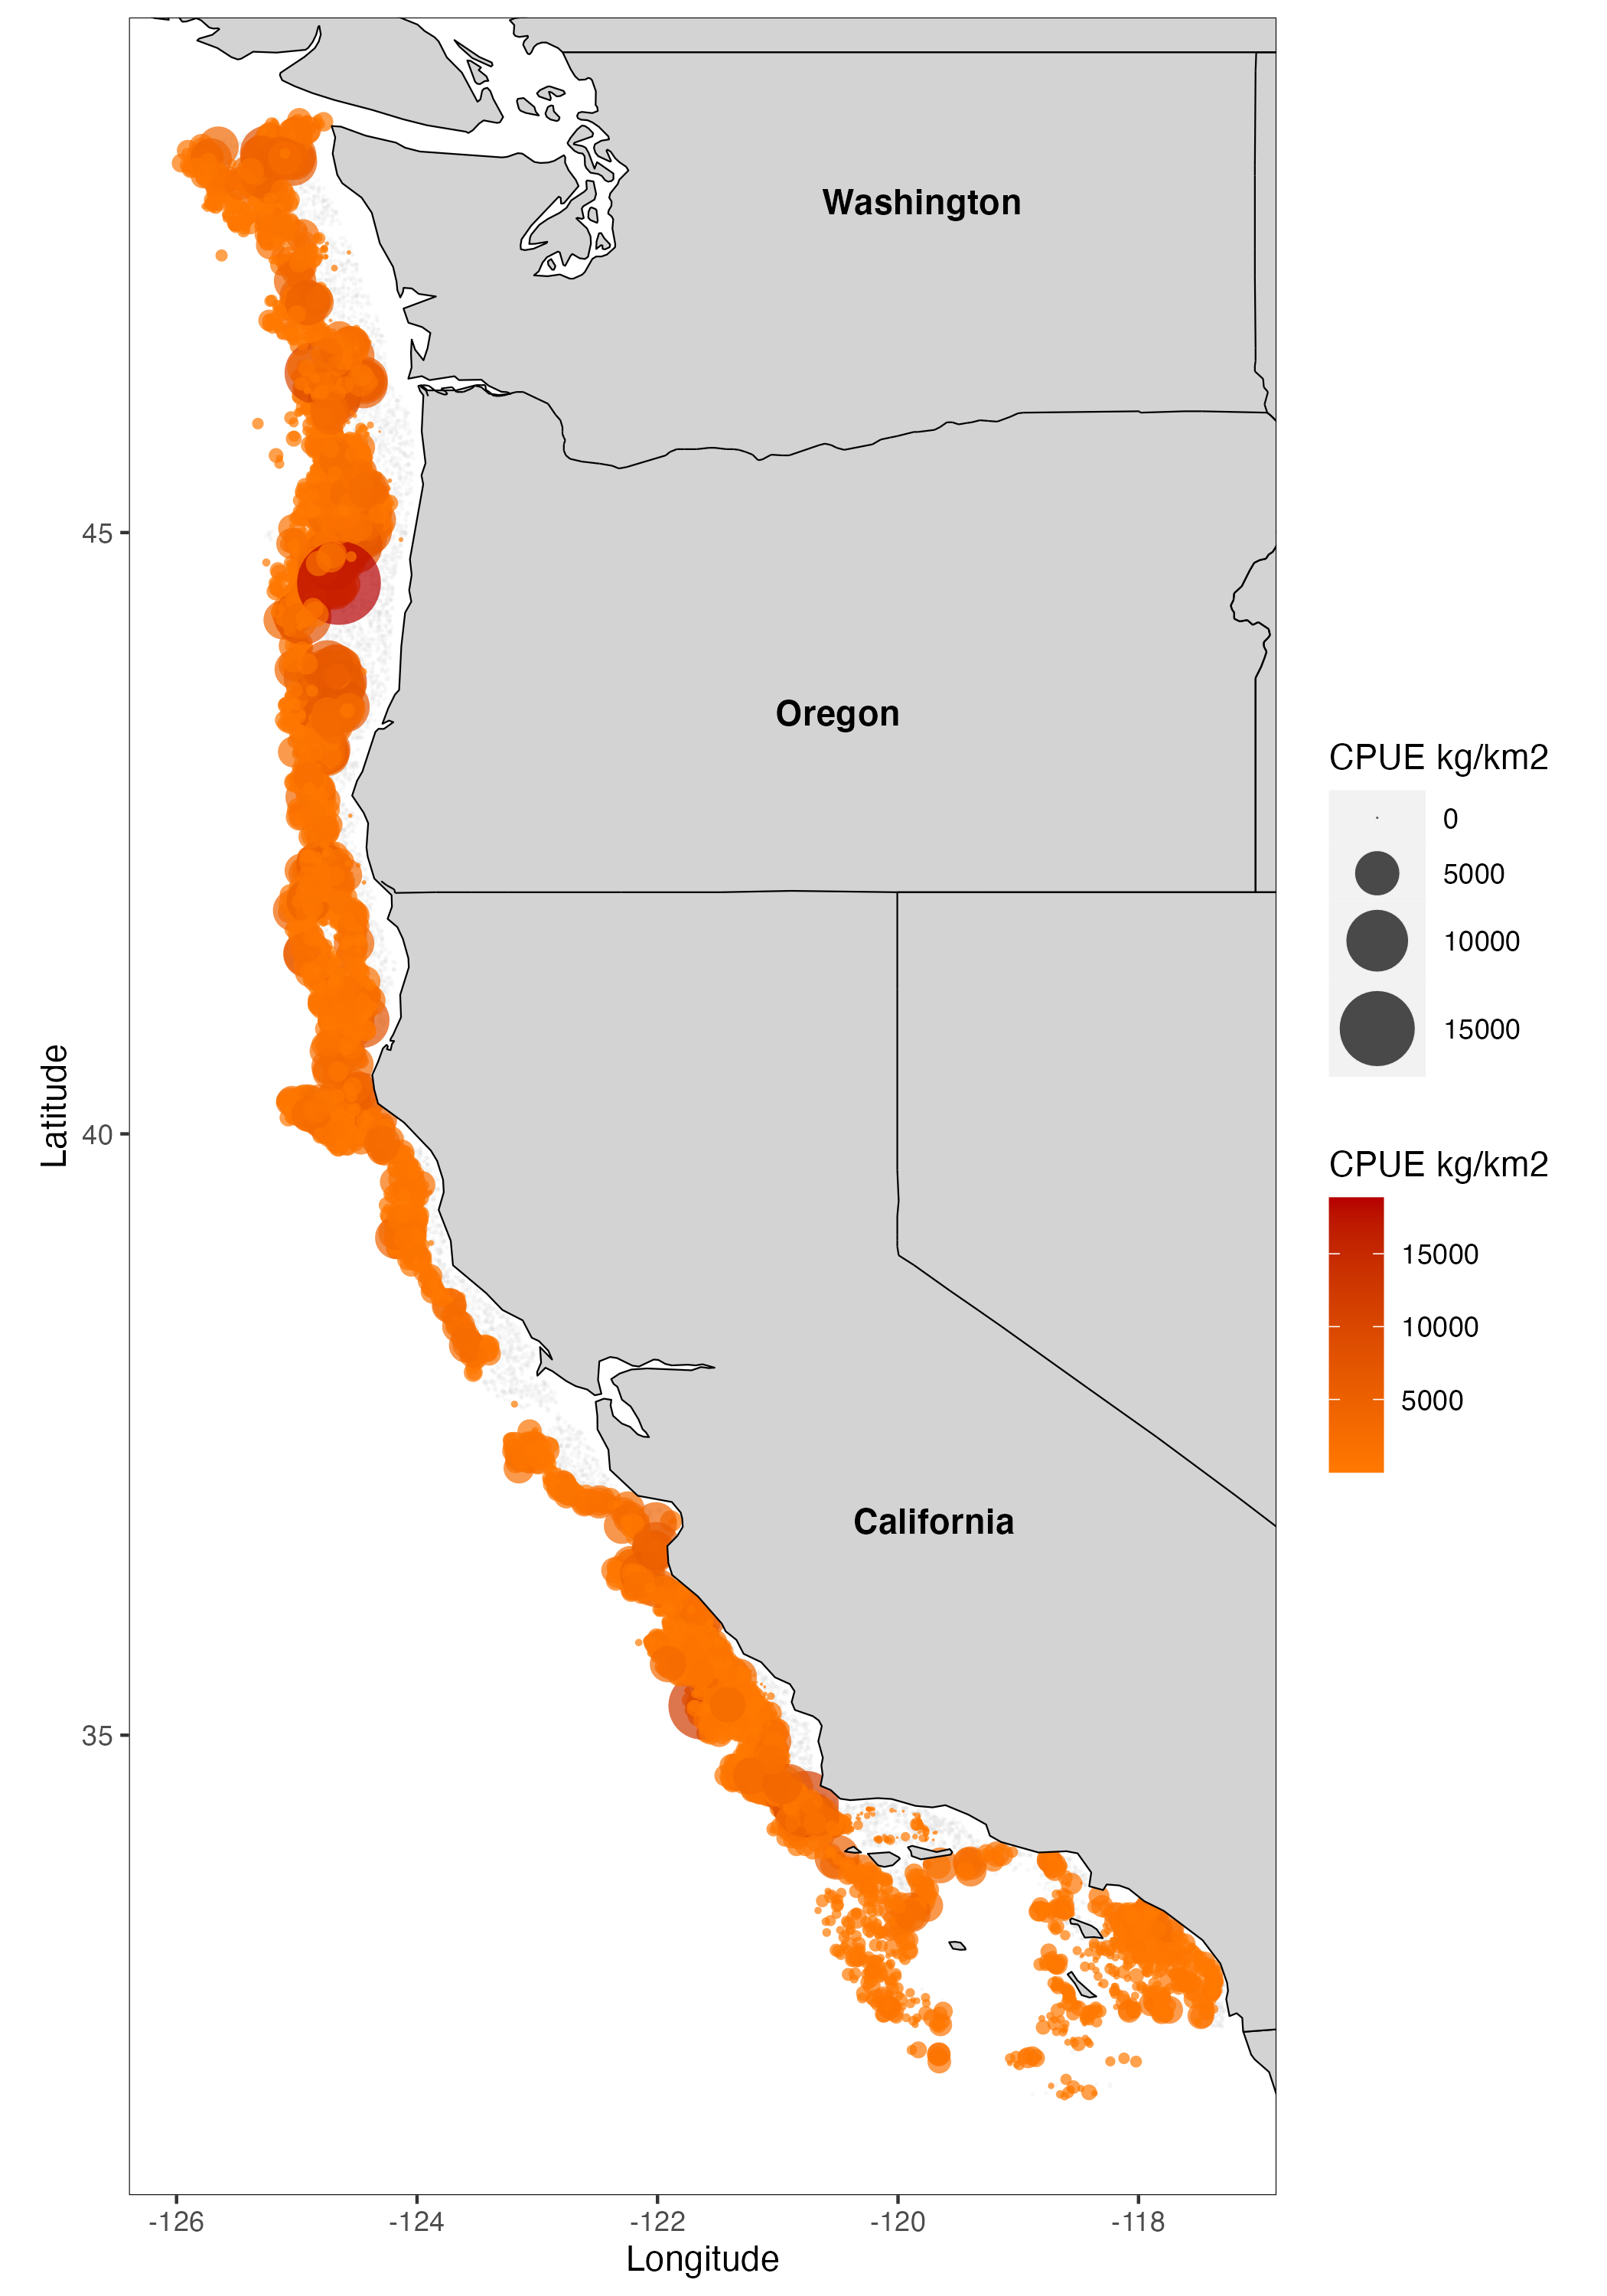
\includegraphics[width=1\textwidth,height=1\textheight]{C:/GitHub/Official_shortspine_thornyhead_2023/doc/FinalFigs/Intro/stock-map.png}
\caption{Biomass of shortspine thornyhead found in the NWFSC West Coast Groundfish Bottom Trawl Survey annual survey (2003-2022) coastwide.\label{fig:stock-map}}
\end{figure}

\begin{figure}
\centering
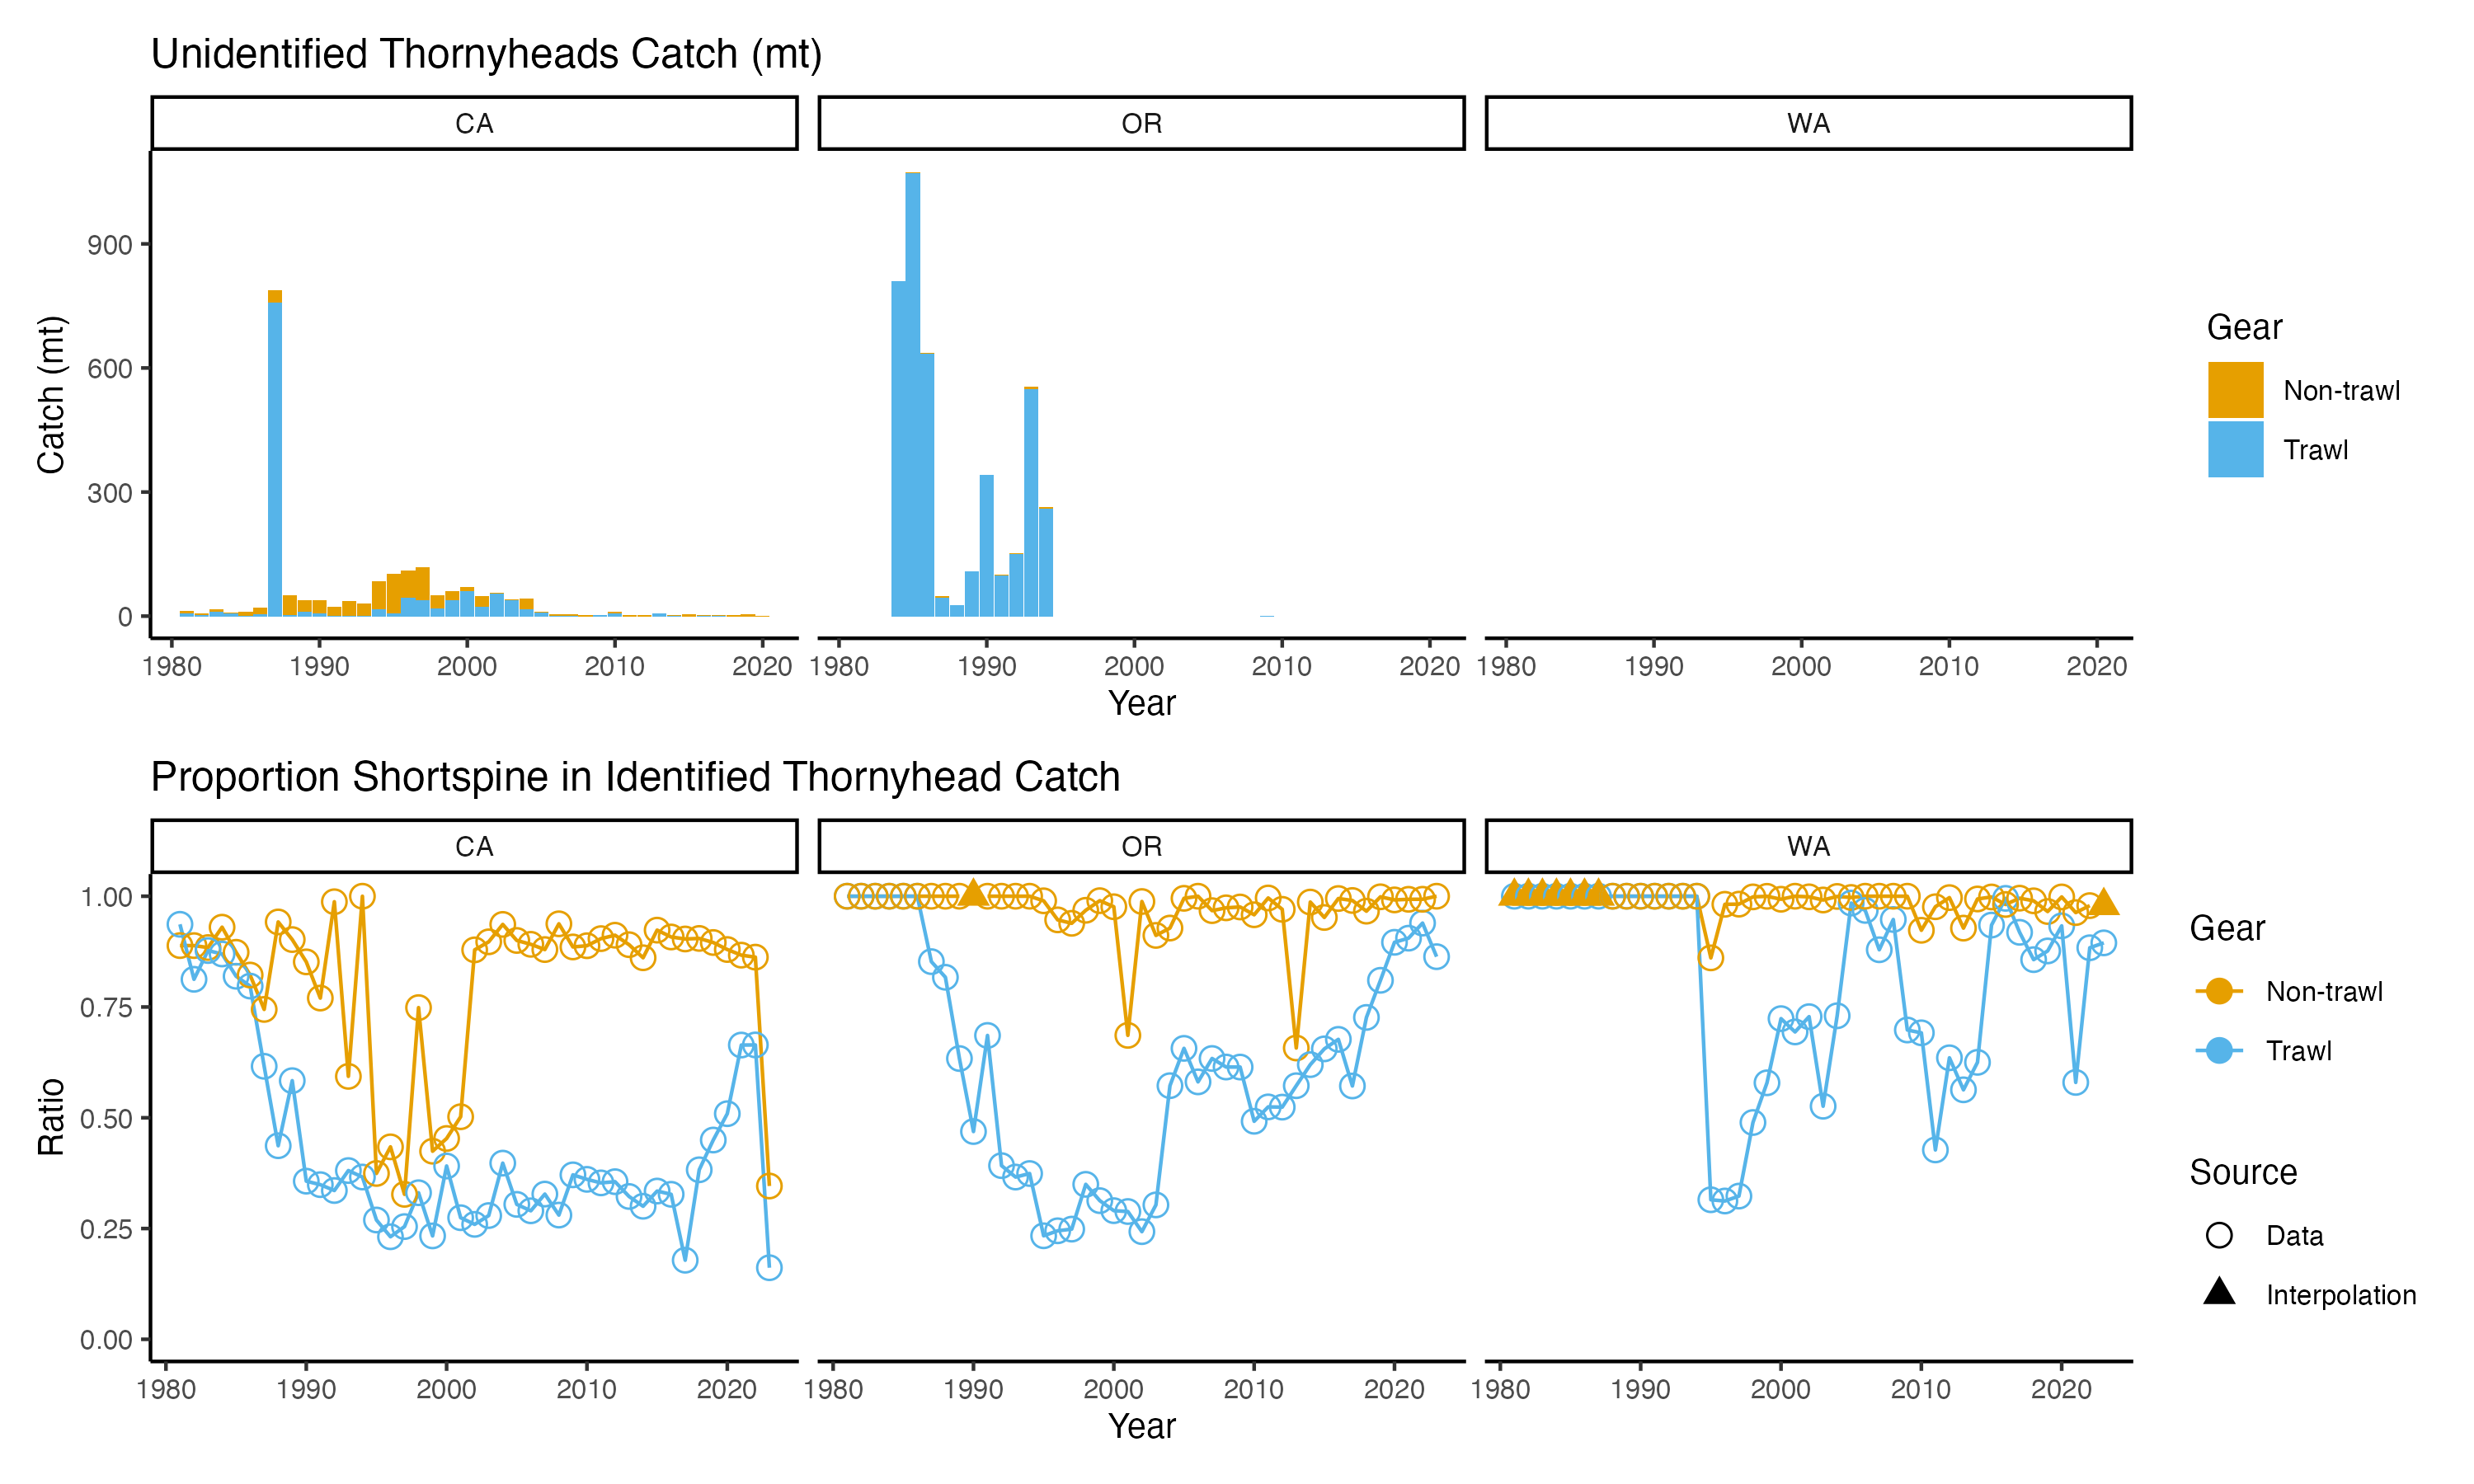
\includegraphics[width=1\textwidth,height=1\textheight]{C:/GitHub/Official_shortspine_thornyhead_2023/doc/FinalFigs/Intro/thornyhead-ratio.png}
\caption{Unidentified thornyhead catches (mt) and the proportion identified as shortspines, calculated as the ratio of shortspine thornyhead catches and longspine and shortspine catches.\label{fig:thornyhead-ratio}}
\end{figure}

\begin{figure}
\centering
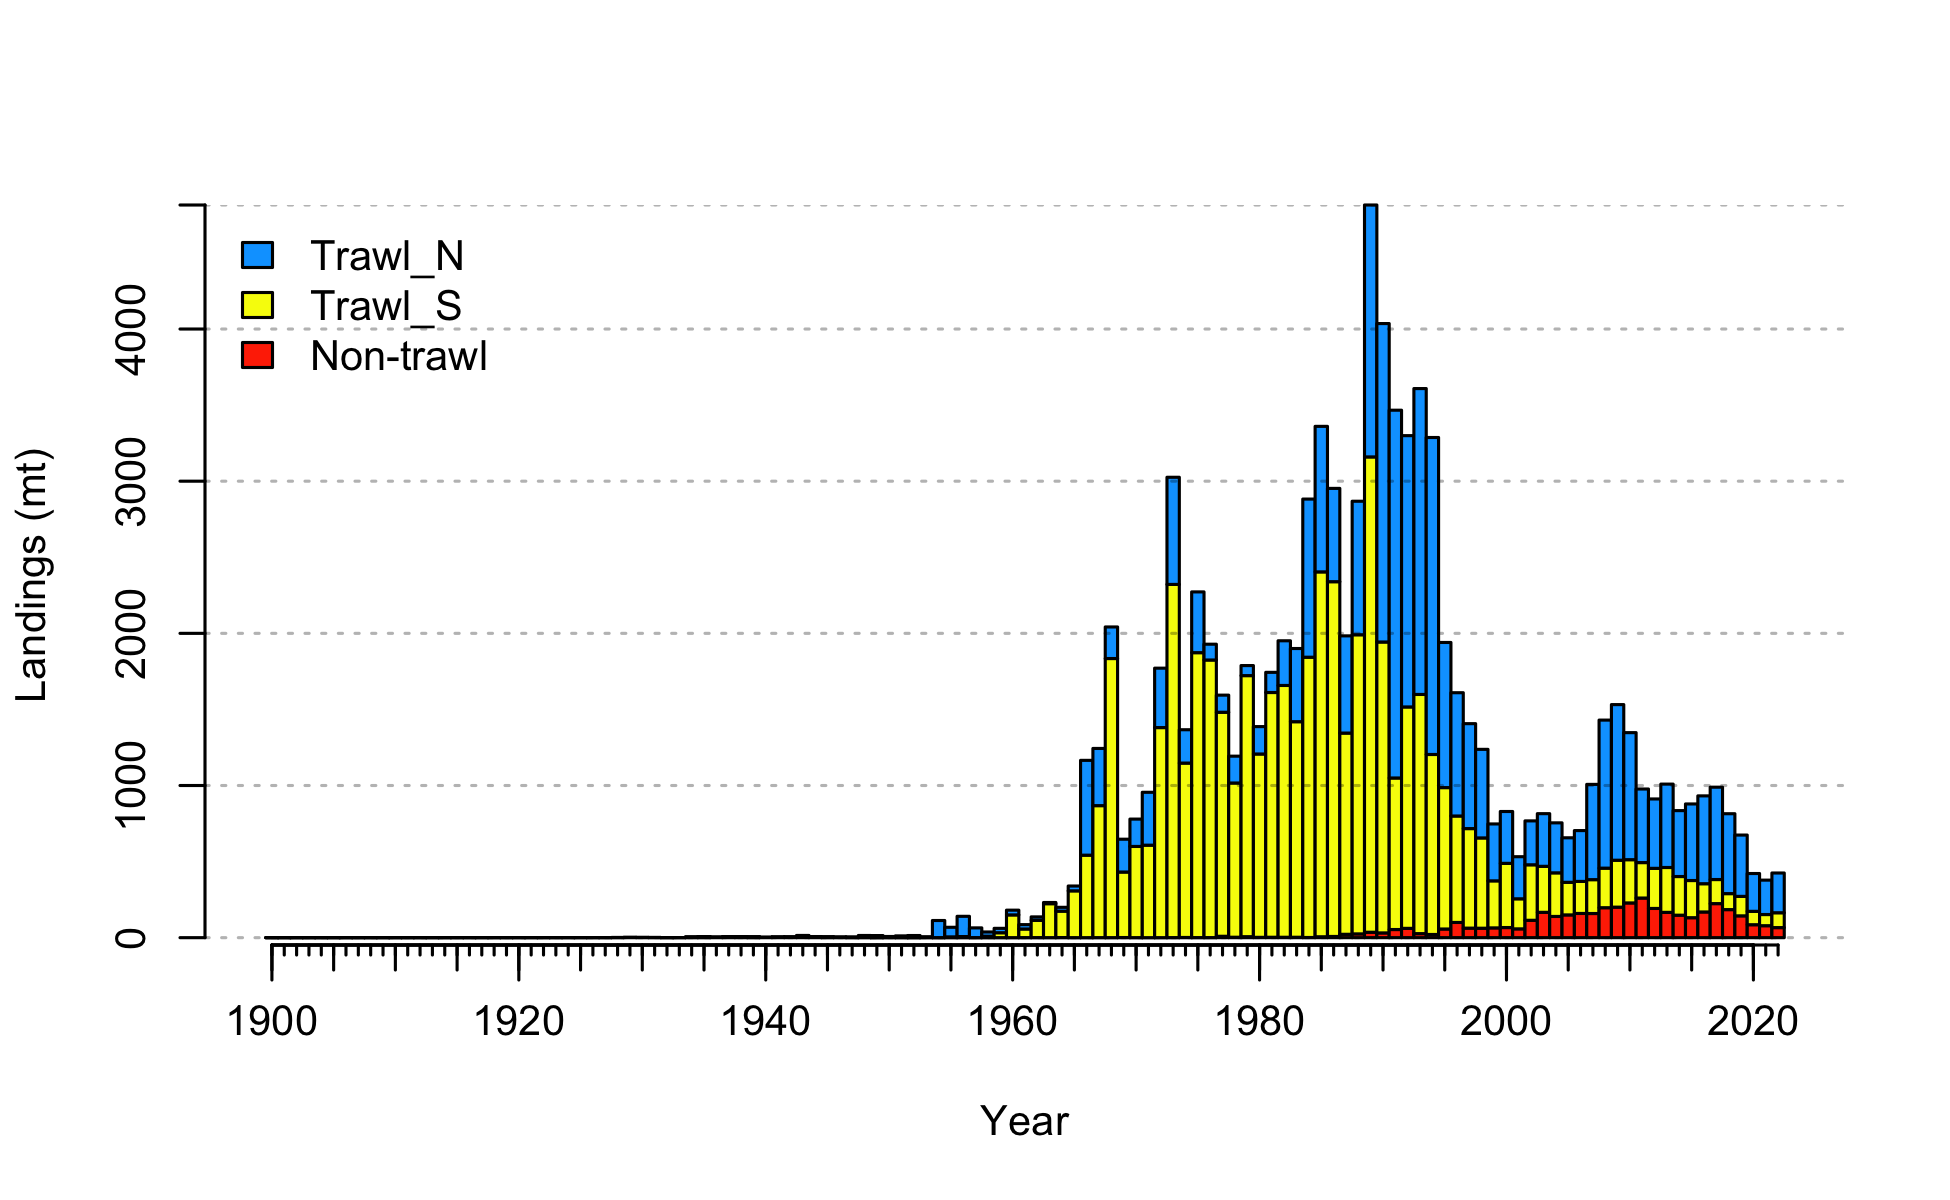
\includegraphics[width=1\textwidth,height=1\textheight]{C:/GitHub/Official_shortspine_thornyhead_2023/doc/FinalFigs/Base/catch2 landings stacked.png}
\caption{Estimated landing history for shortspine thornyhead.\label{fig:catch_hist}}
\end{figure}

\begin{figure}
\centering
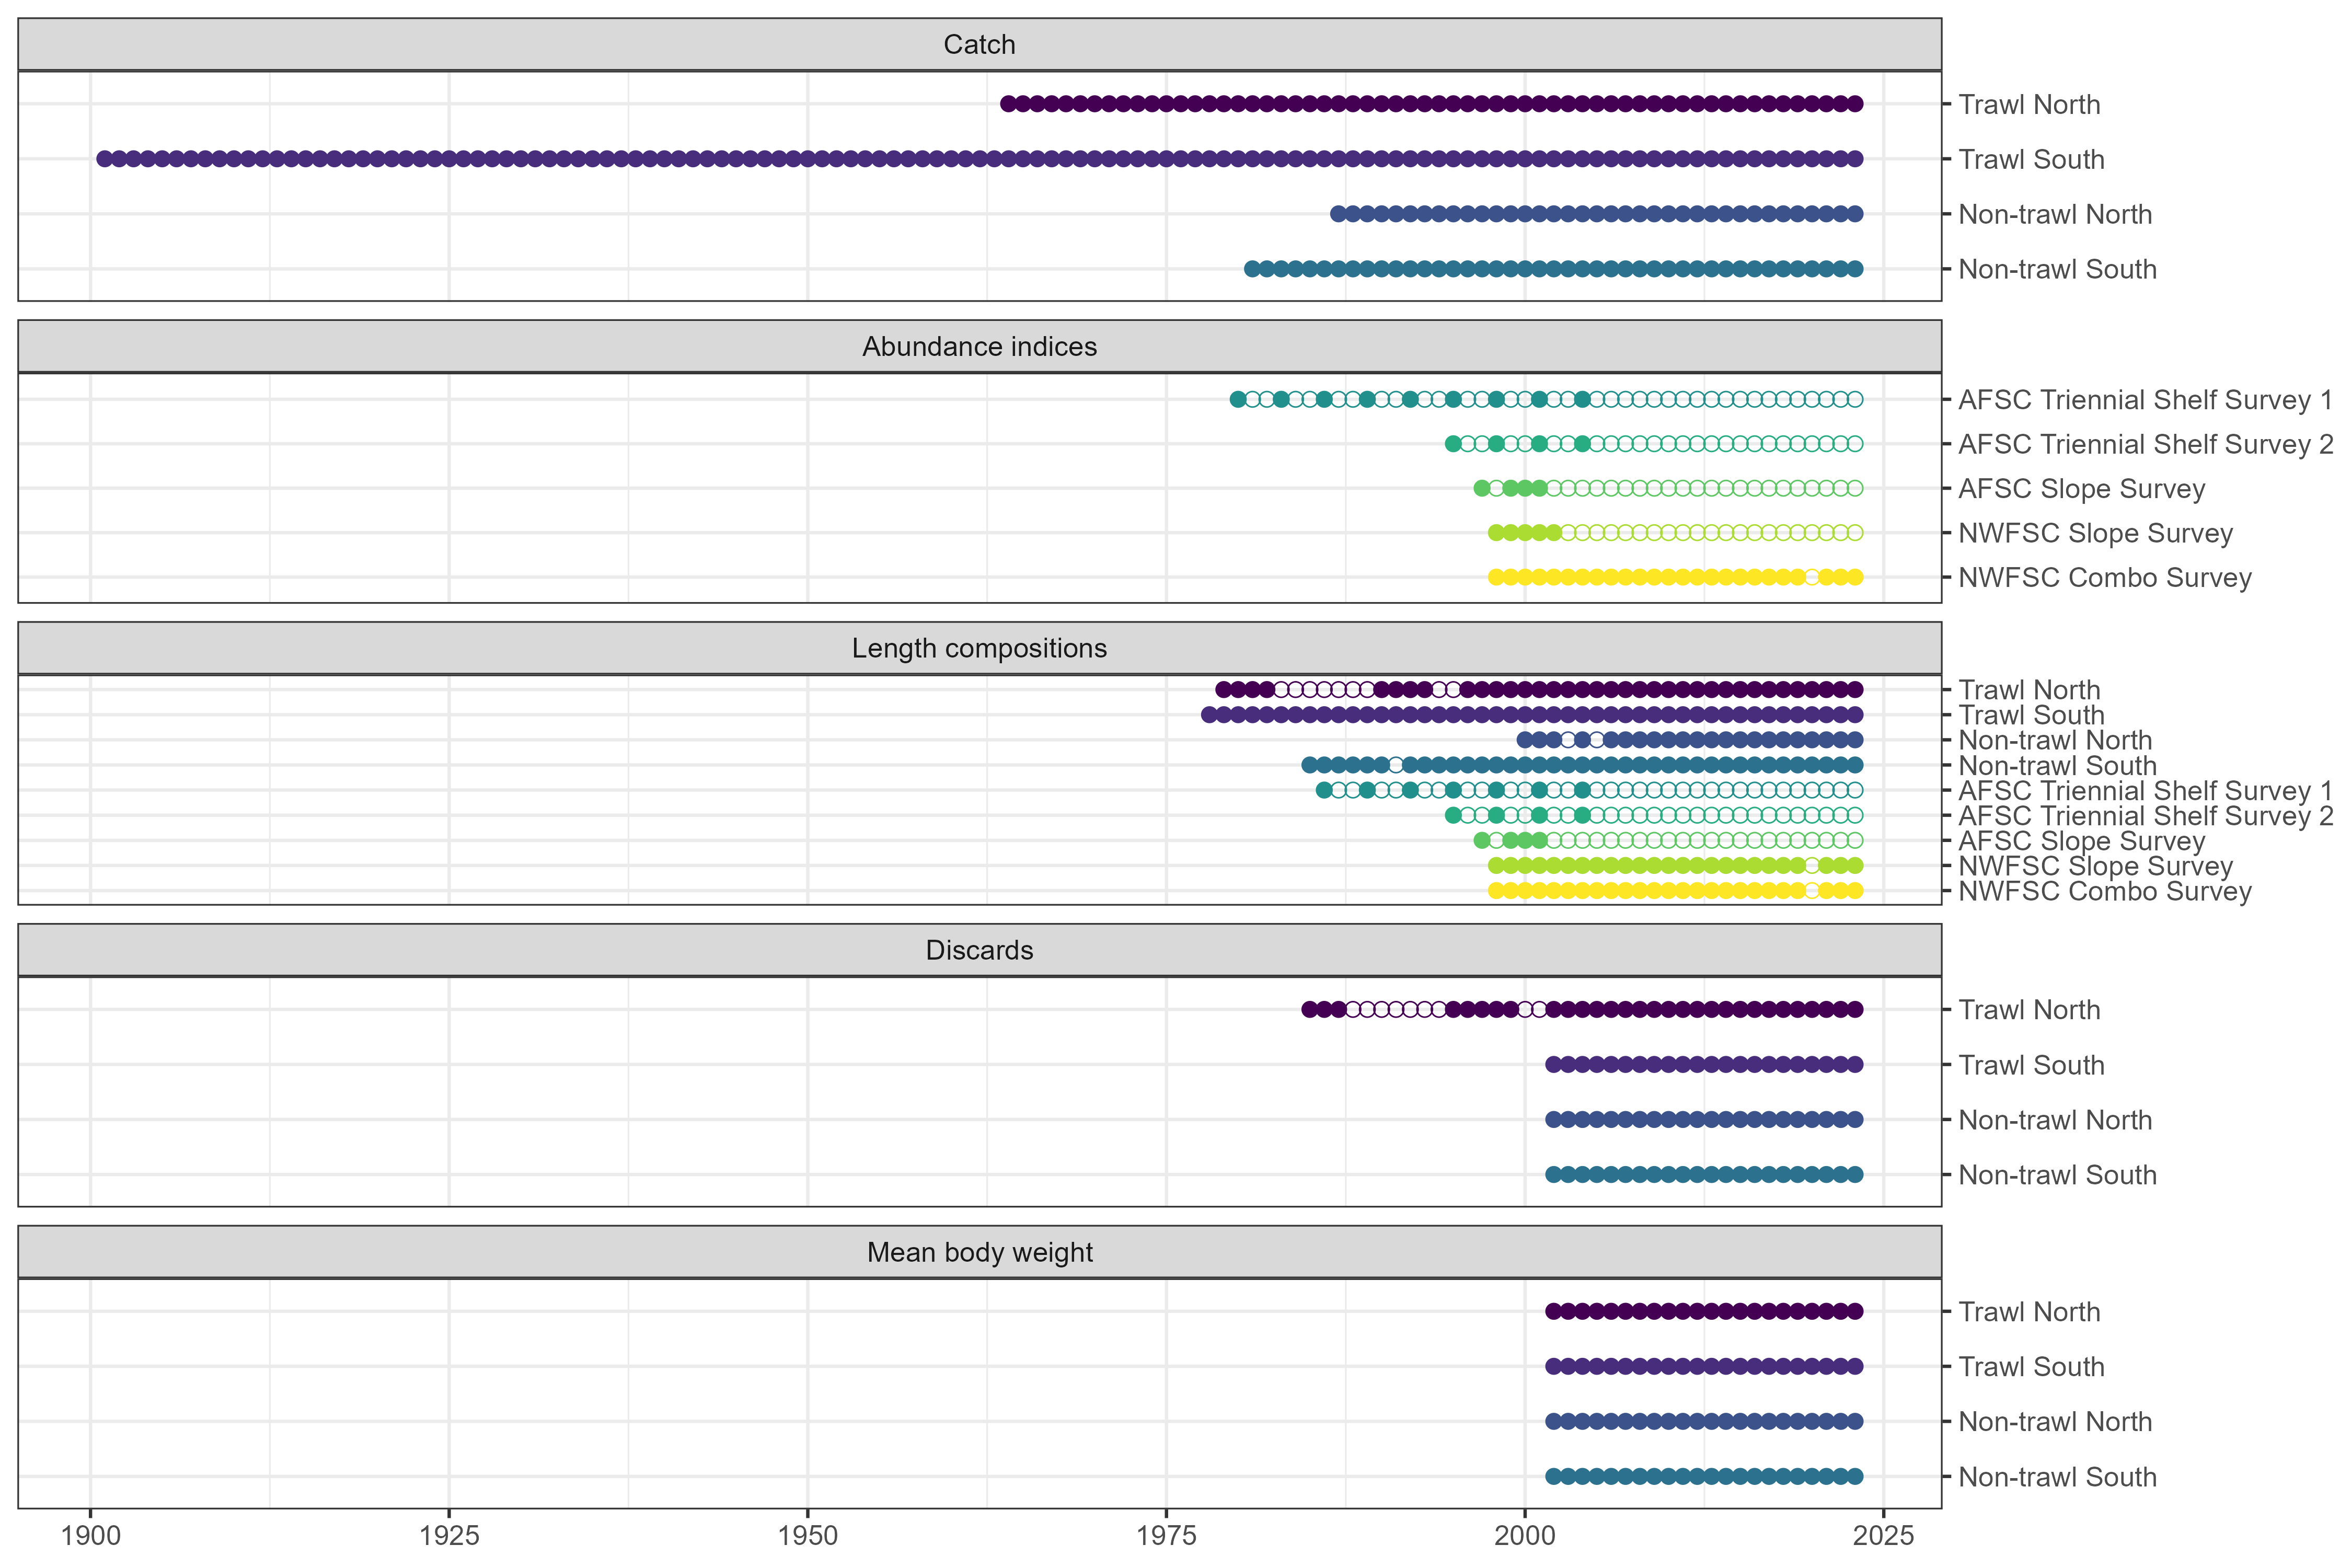
\includegraphics[width=1\textwidth,height=1\textheight]{C:/GitHub/Official_shortspine_thornyhead_2023/doc/FinalFigs/Data/assessment_data_timeseries.png}
\caption{Summary of data sources used in the base model.\label{fig:assessment_data_timeseries}}
\end{figure}

\begin{figure}
\centering
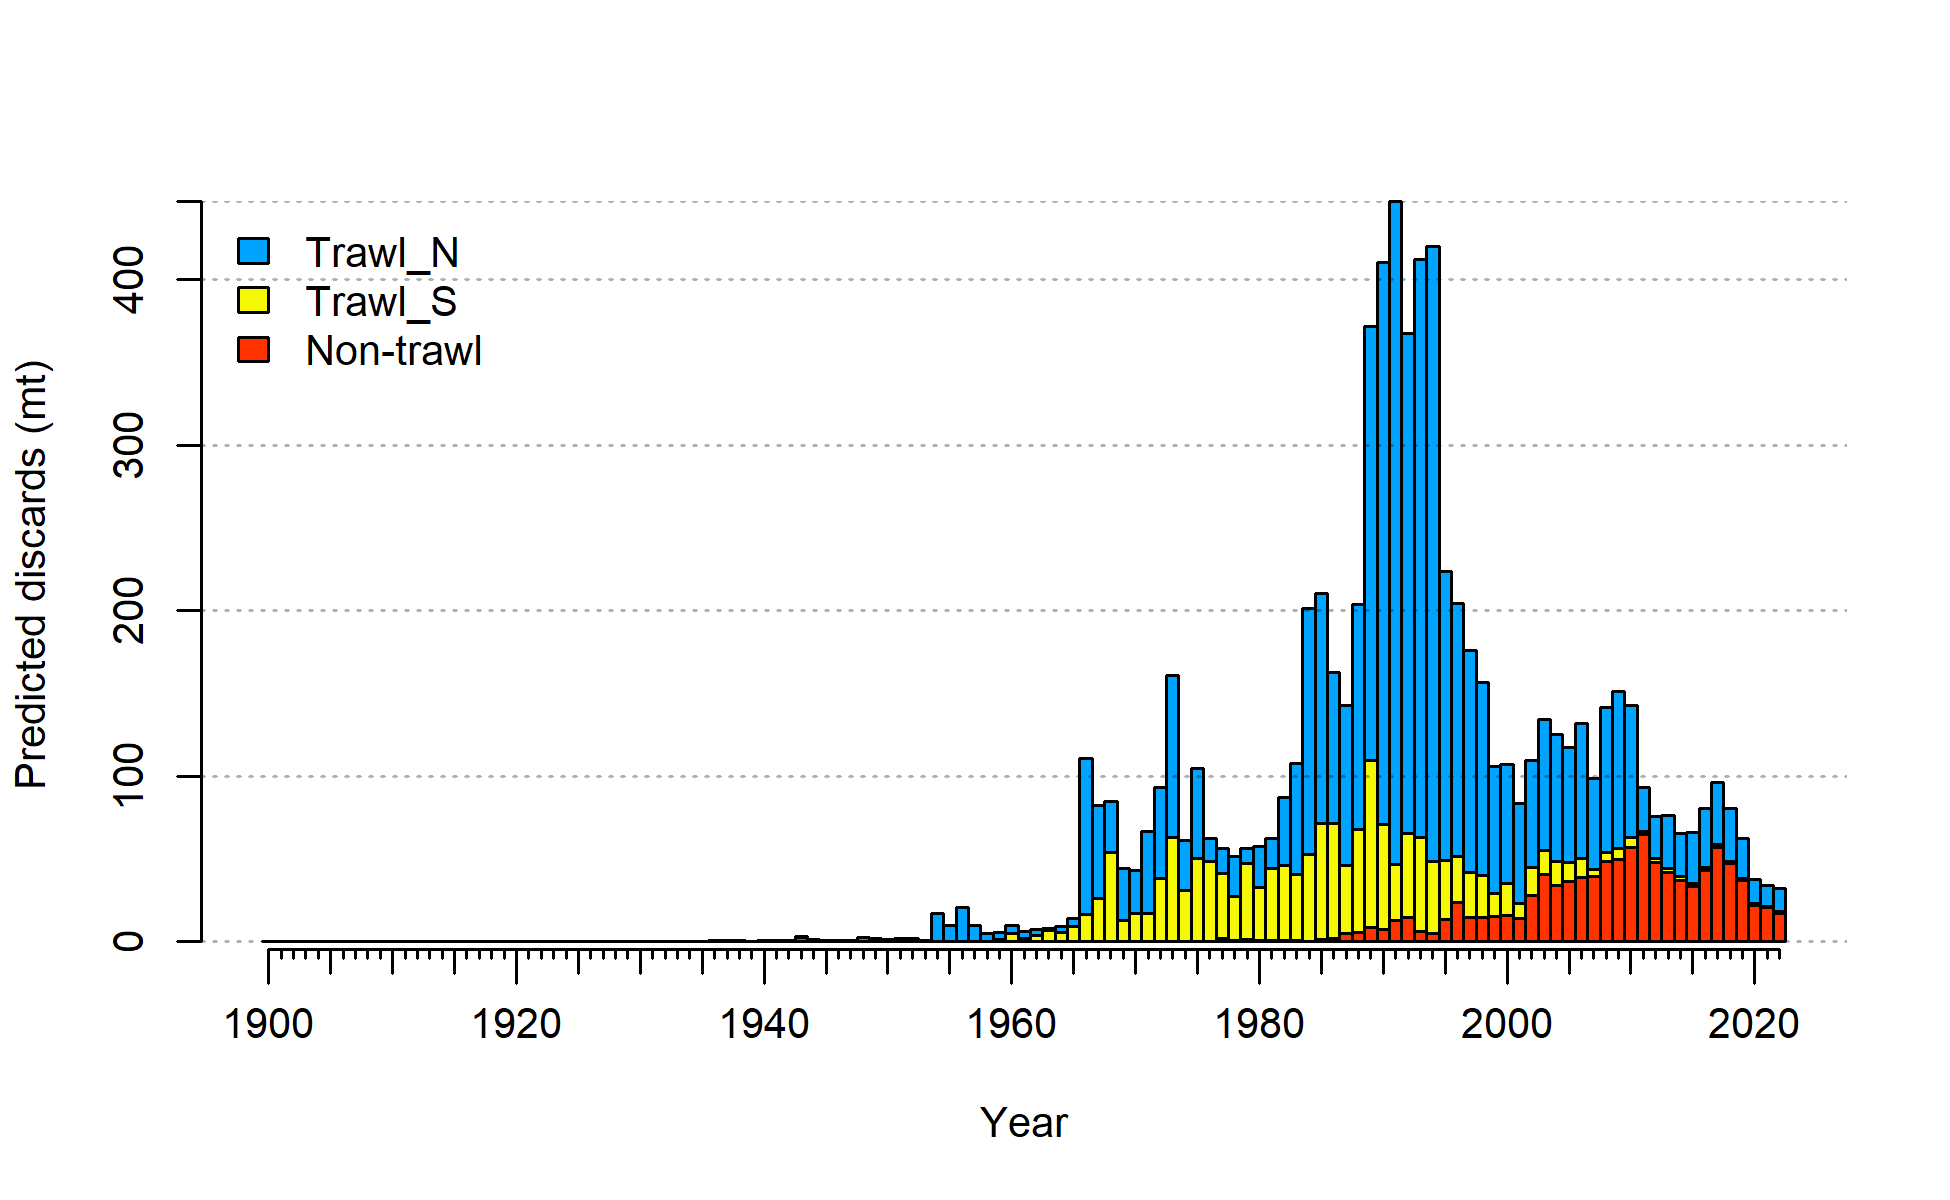
\includegraphics[width=1\textwidth,height=1\textheight]{C:/GitHub/Official_shortspine_thornyhead_2023/doc/FinalFigs/Base/catch7 discards stacked plot (depends on multiple fleets).png}
\caption{Predicted discards based estimated retention and selectivity for each fleet.\label{fig:disc_hist}}
\end{figure}

\begin{figure}
\centering
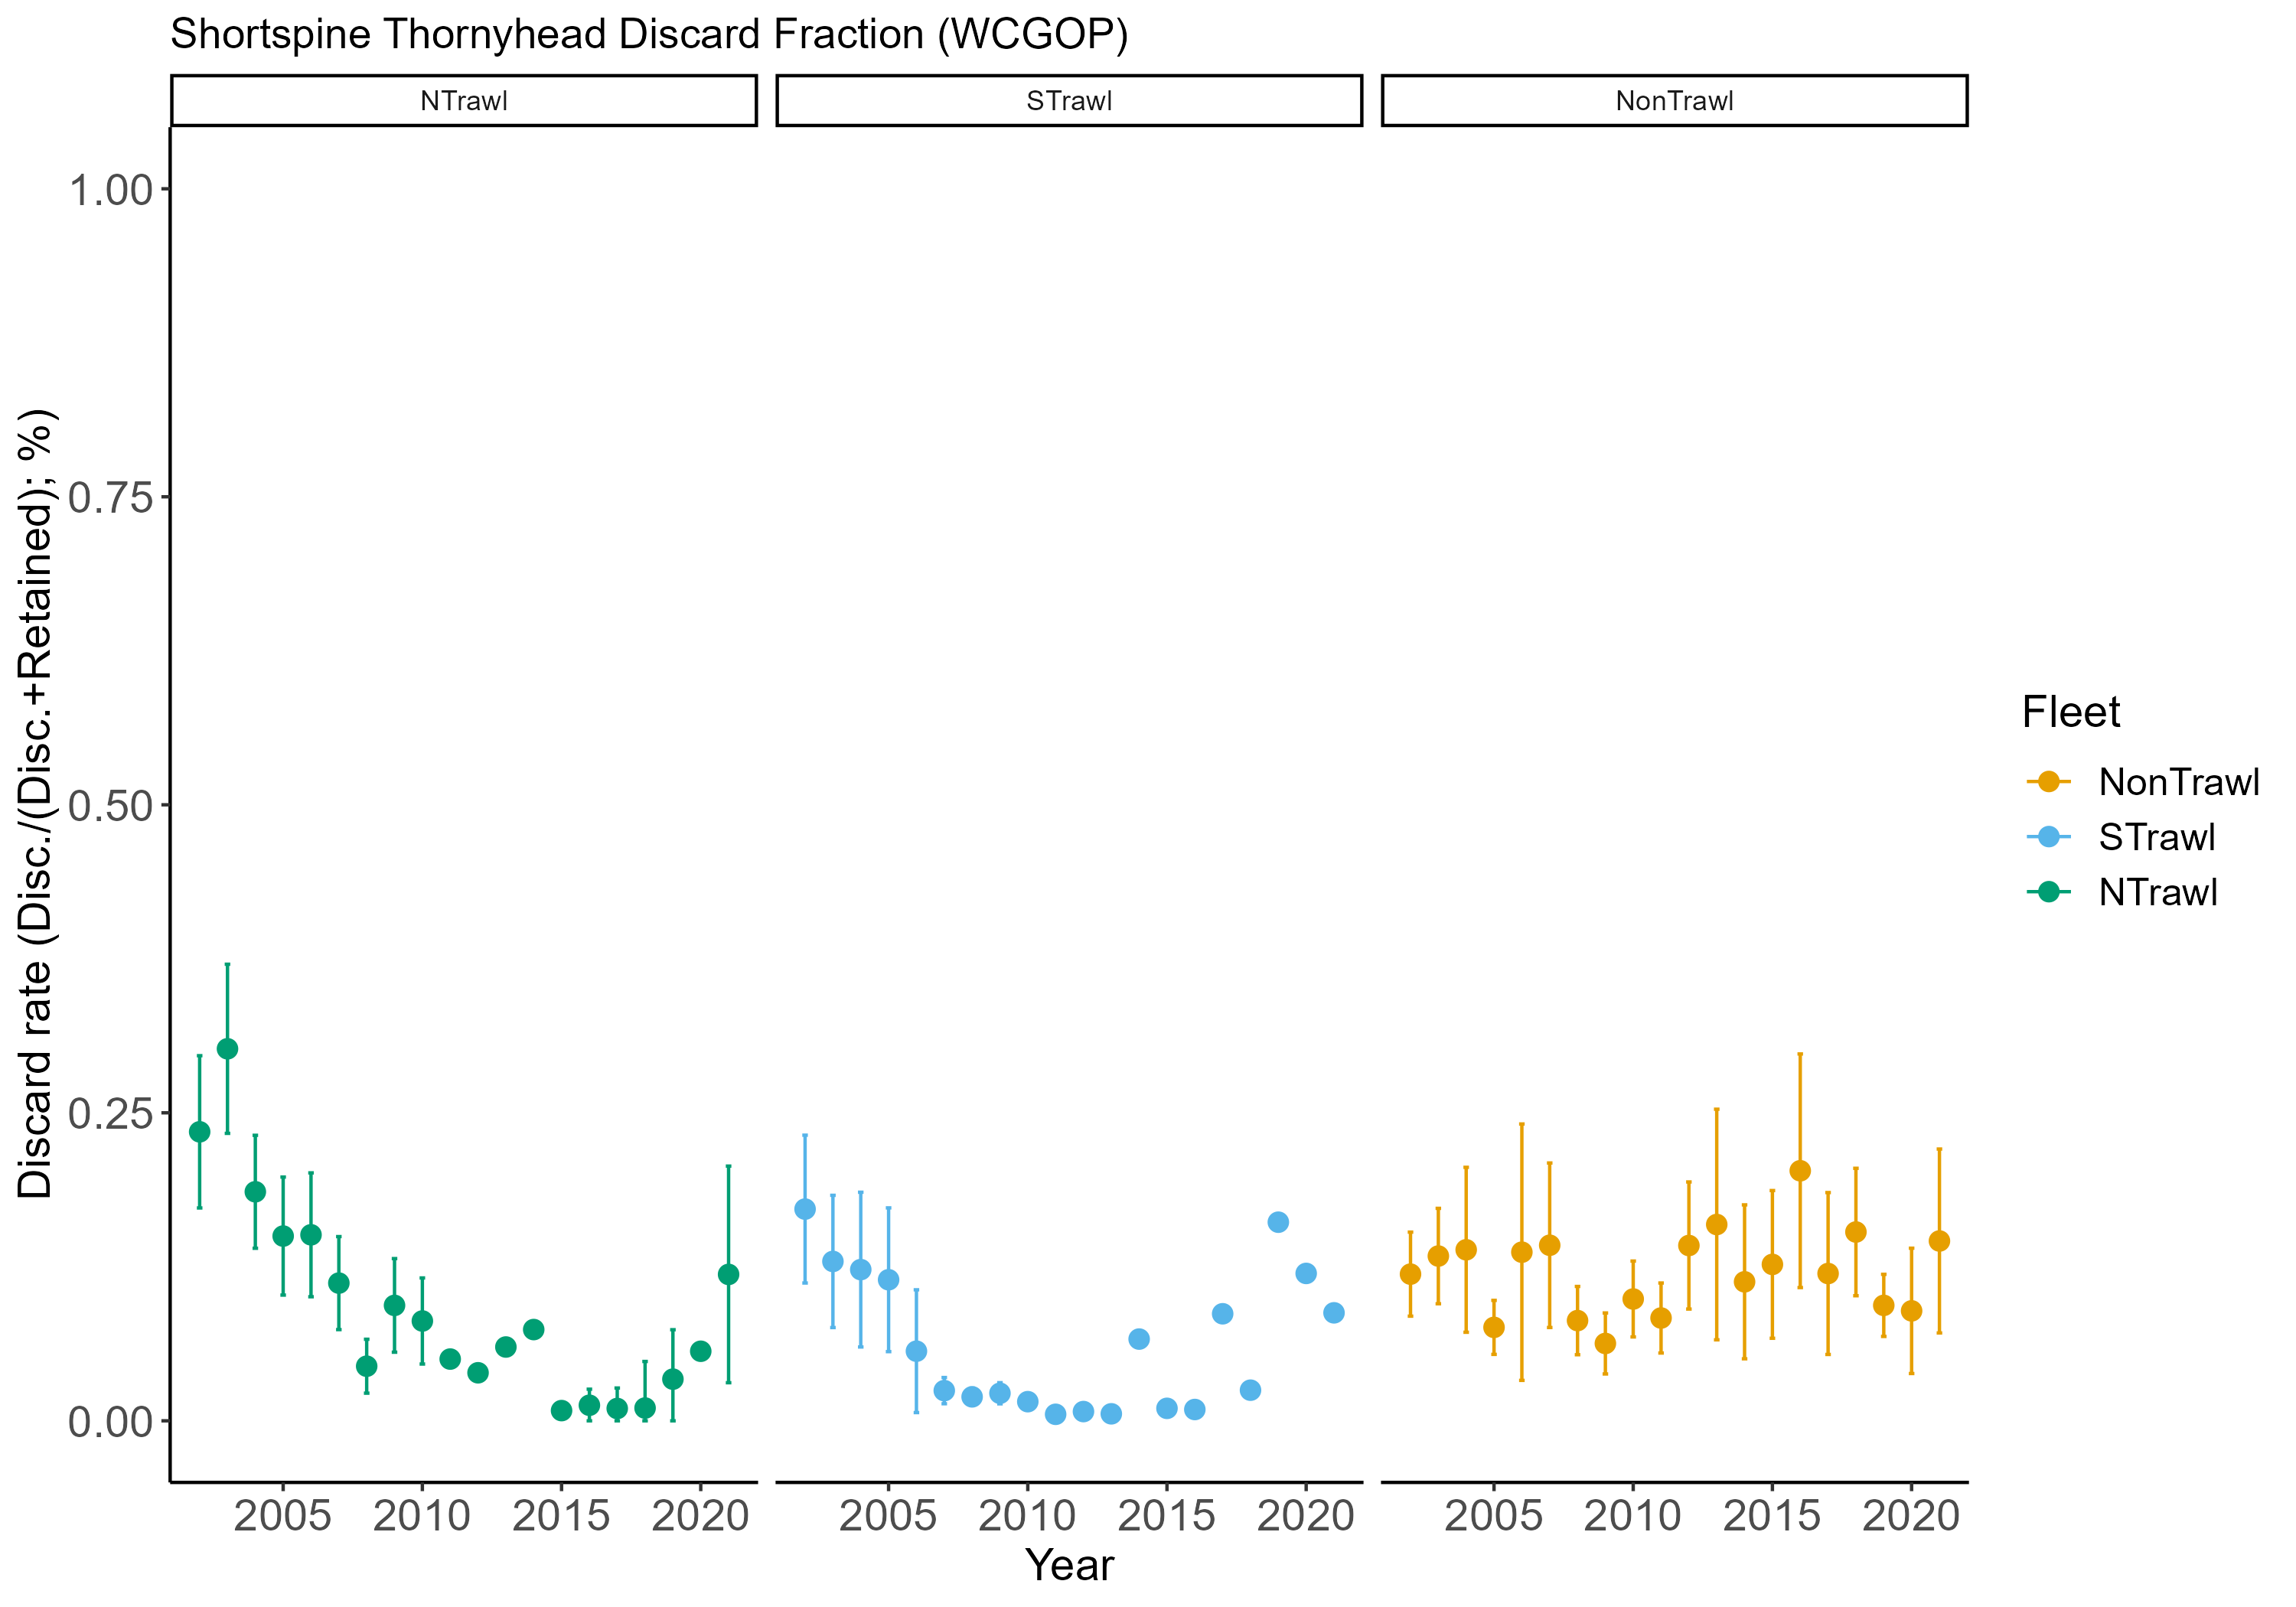
\includegraphics[width=1\textwidth,height=1\textheight]{C:/GitHub/Official_shortspine_thornyhead_2023/doc/FinalFigs/Data/SST_WCGOP_GEMM_discard_rates_3fleet.png}
\caption{Discard rates from the WCGOP data set with catch share and non-catch share considerations from the GEMM dataset.\label{fig:disc_rates_WCGOP}}
\end{figure}

\begin{figure}
\centering
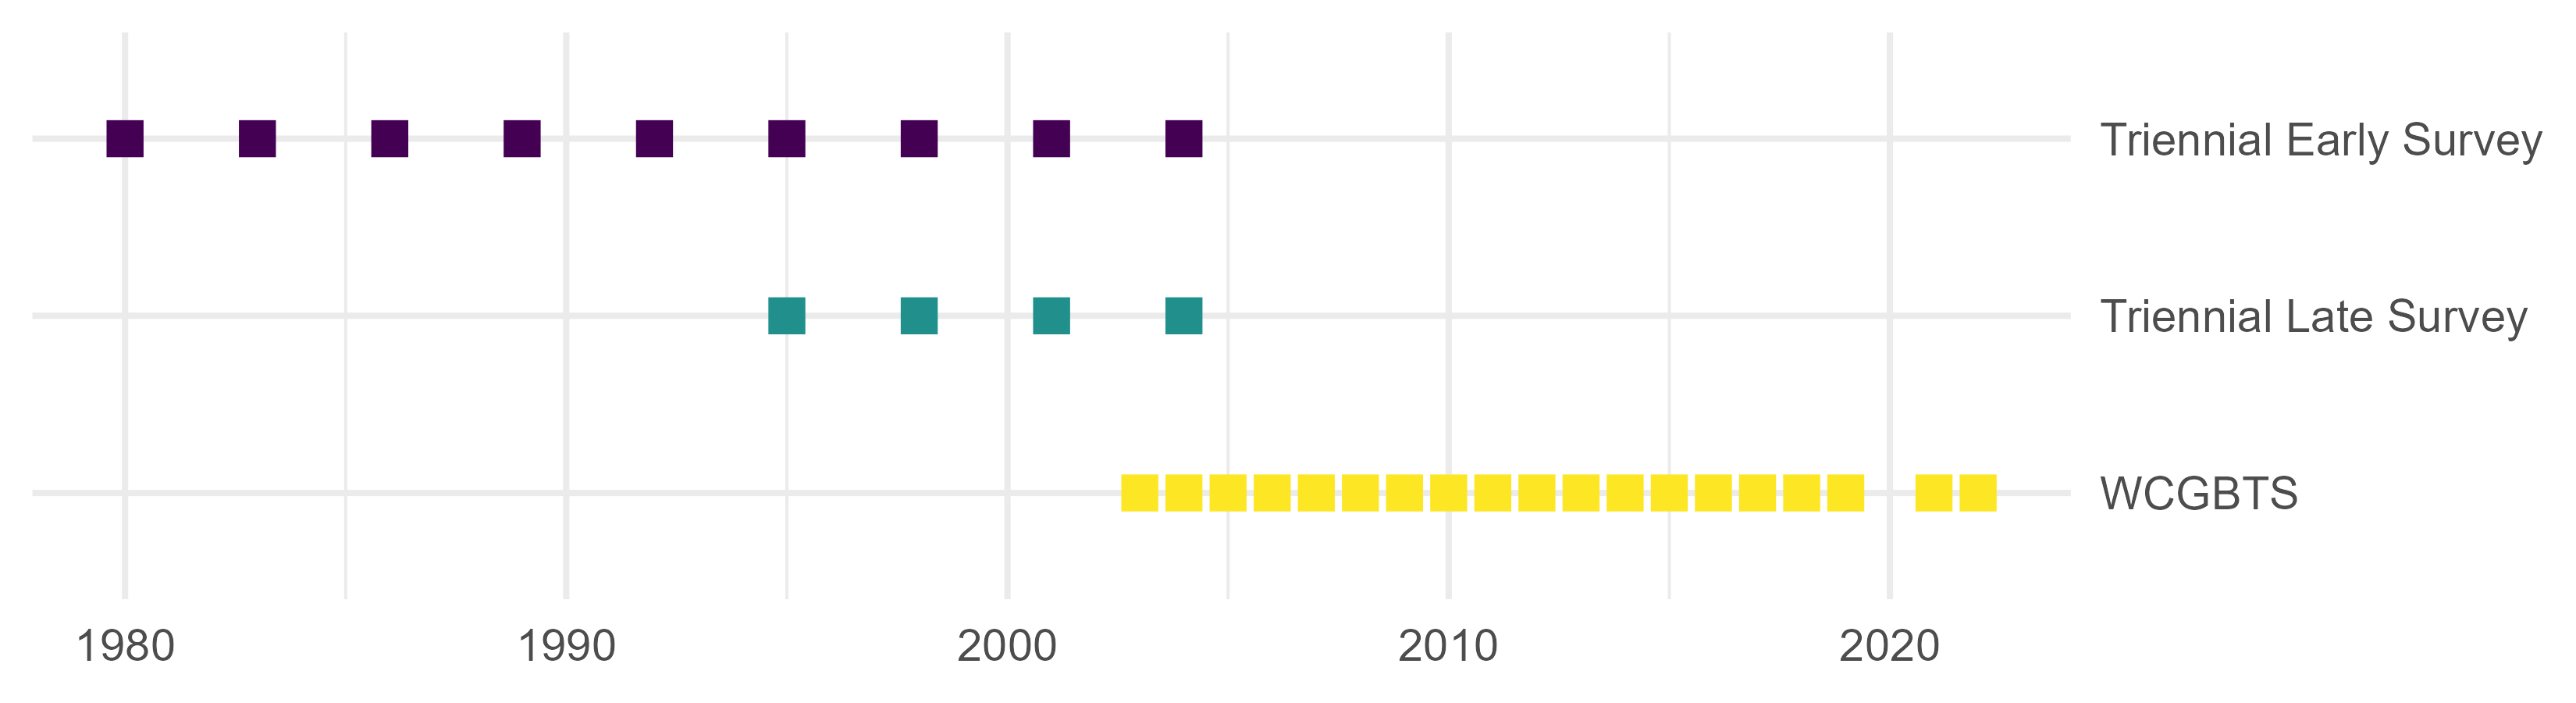
\includegraphics[width=1\textwidth,height=1\textheight]{C:/GitHub/Official_shortspine_thornyhead_2023/doc/FinalFigs/Data/survey_data_timeseries.png}
\caption{Summary of survey data sources used in the base model.\label{fig:survey_data_timeseries}}
\end{figure}

\begin{figure}
\centering
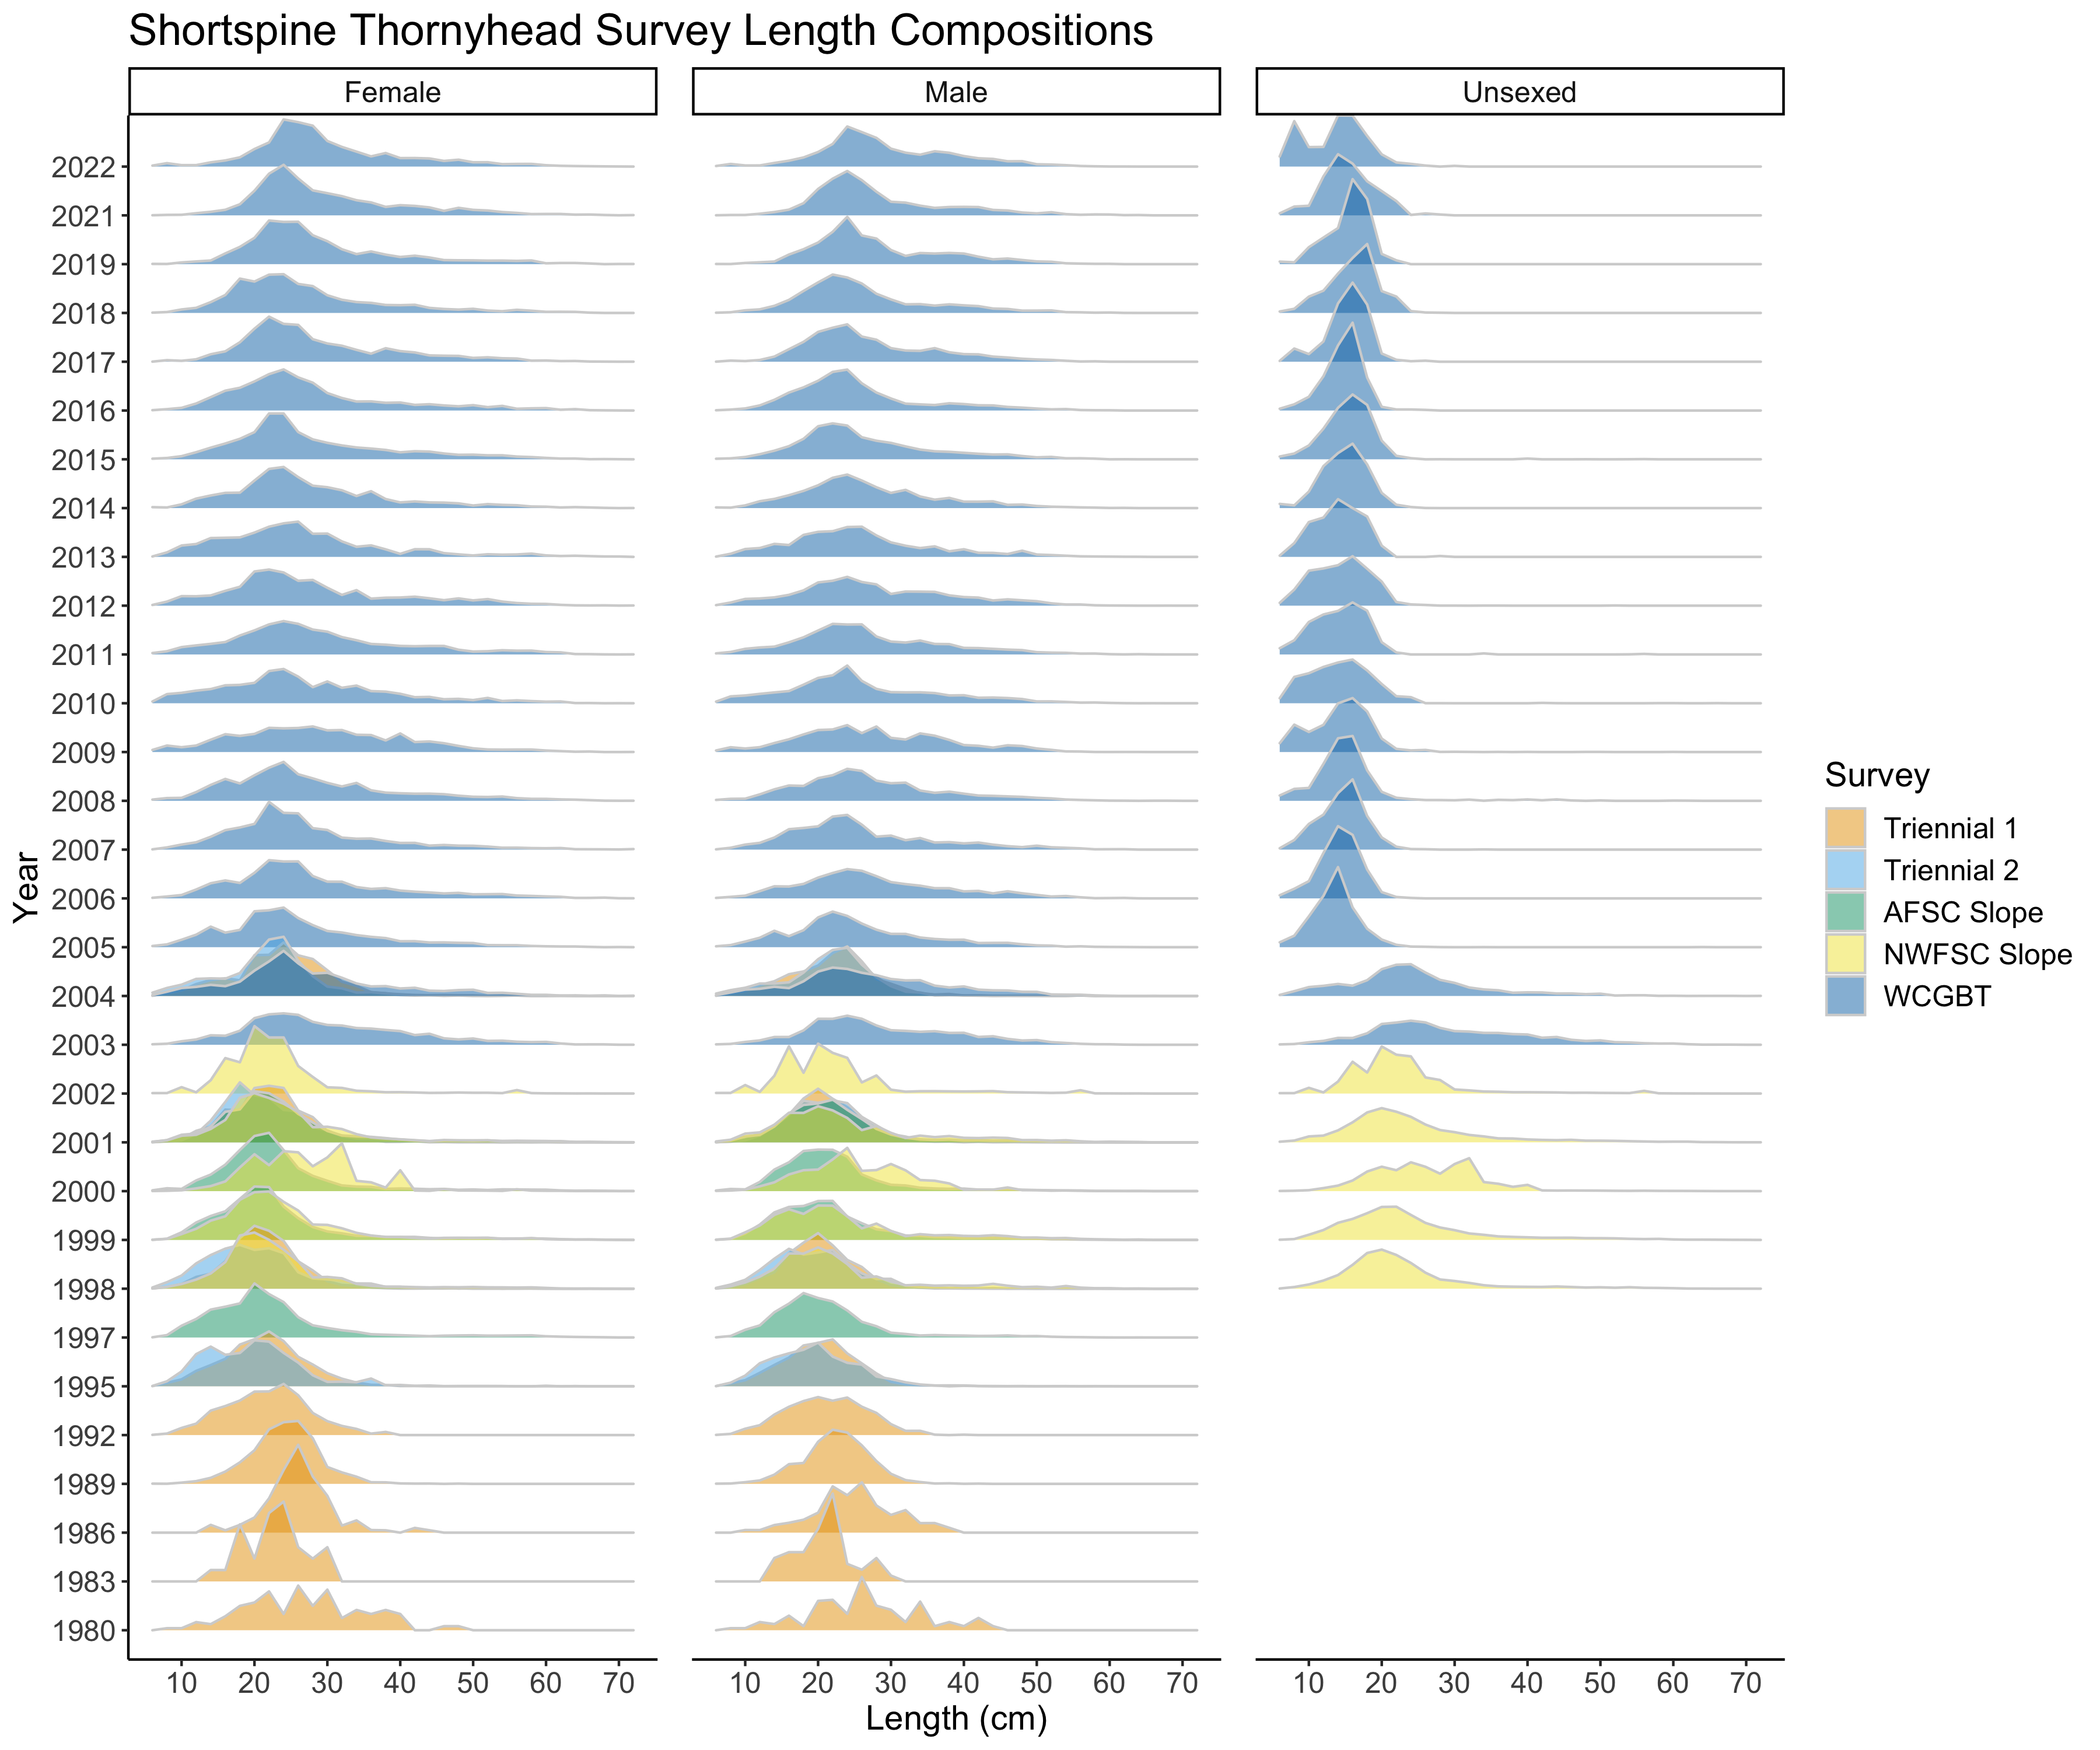
\includegraphics[width=1\textwidth,height=1\textheight]{C:/GitHub/Official_shortspine_thornyhead_2023/doc/FinalFigs/Data/2023_length_compositions.png}
\caption{Survey length composition data.\label{fig:survey_comps}}
\end{figure}

\begin{figure}
\centering
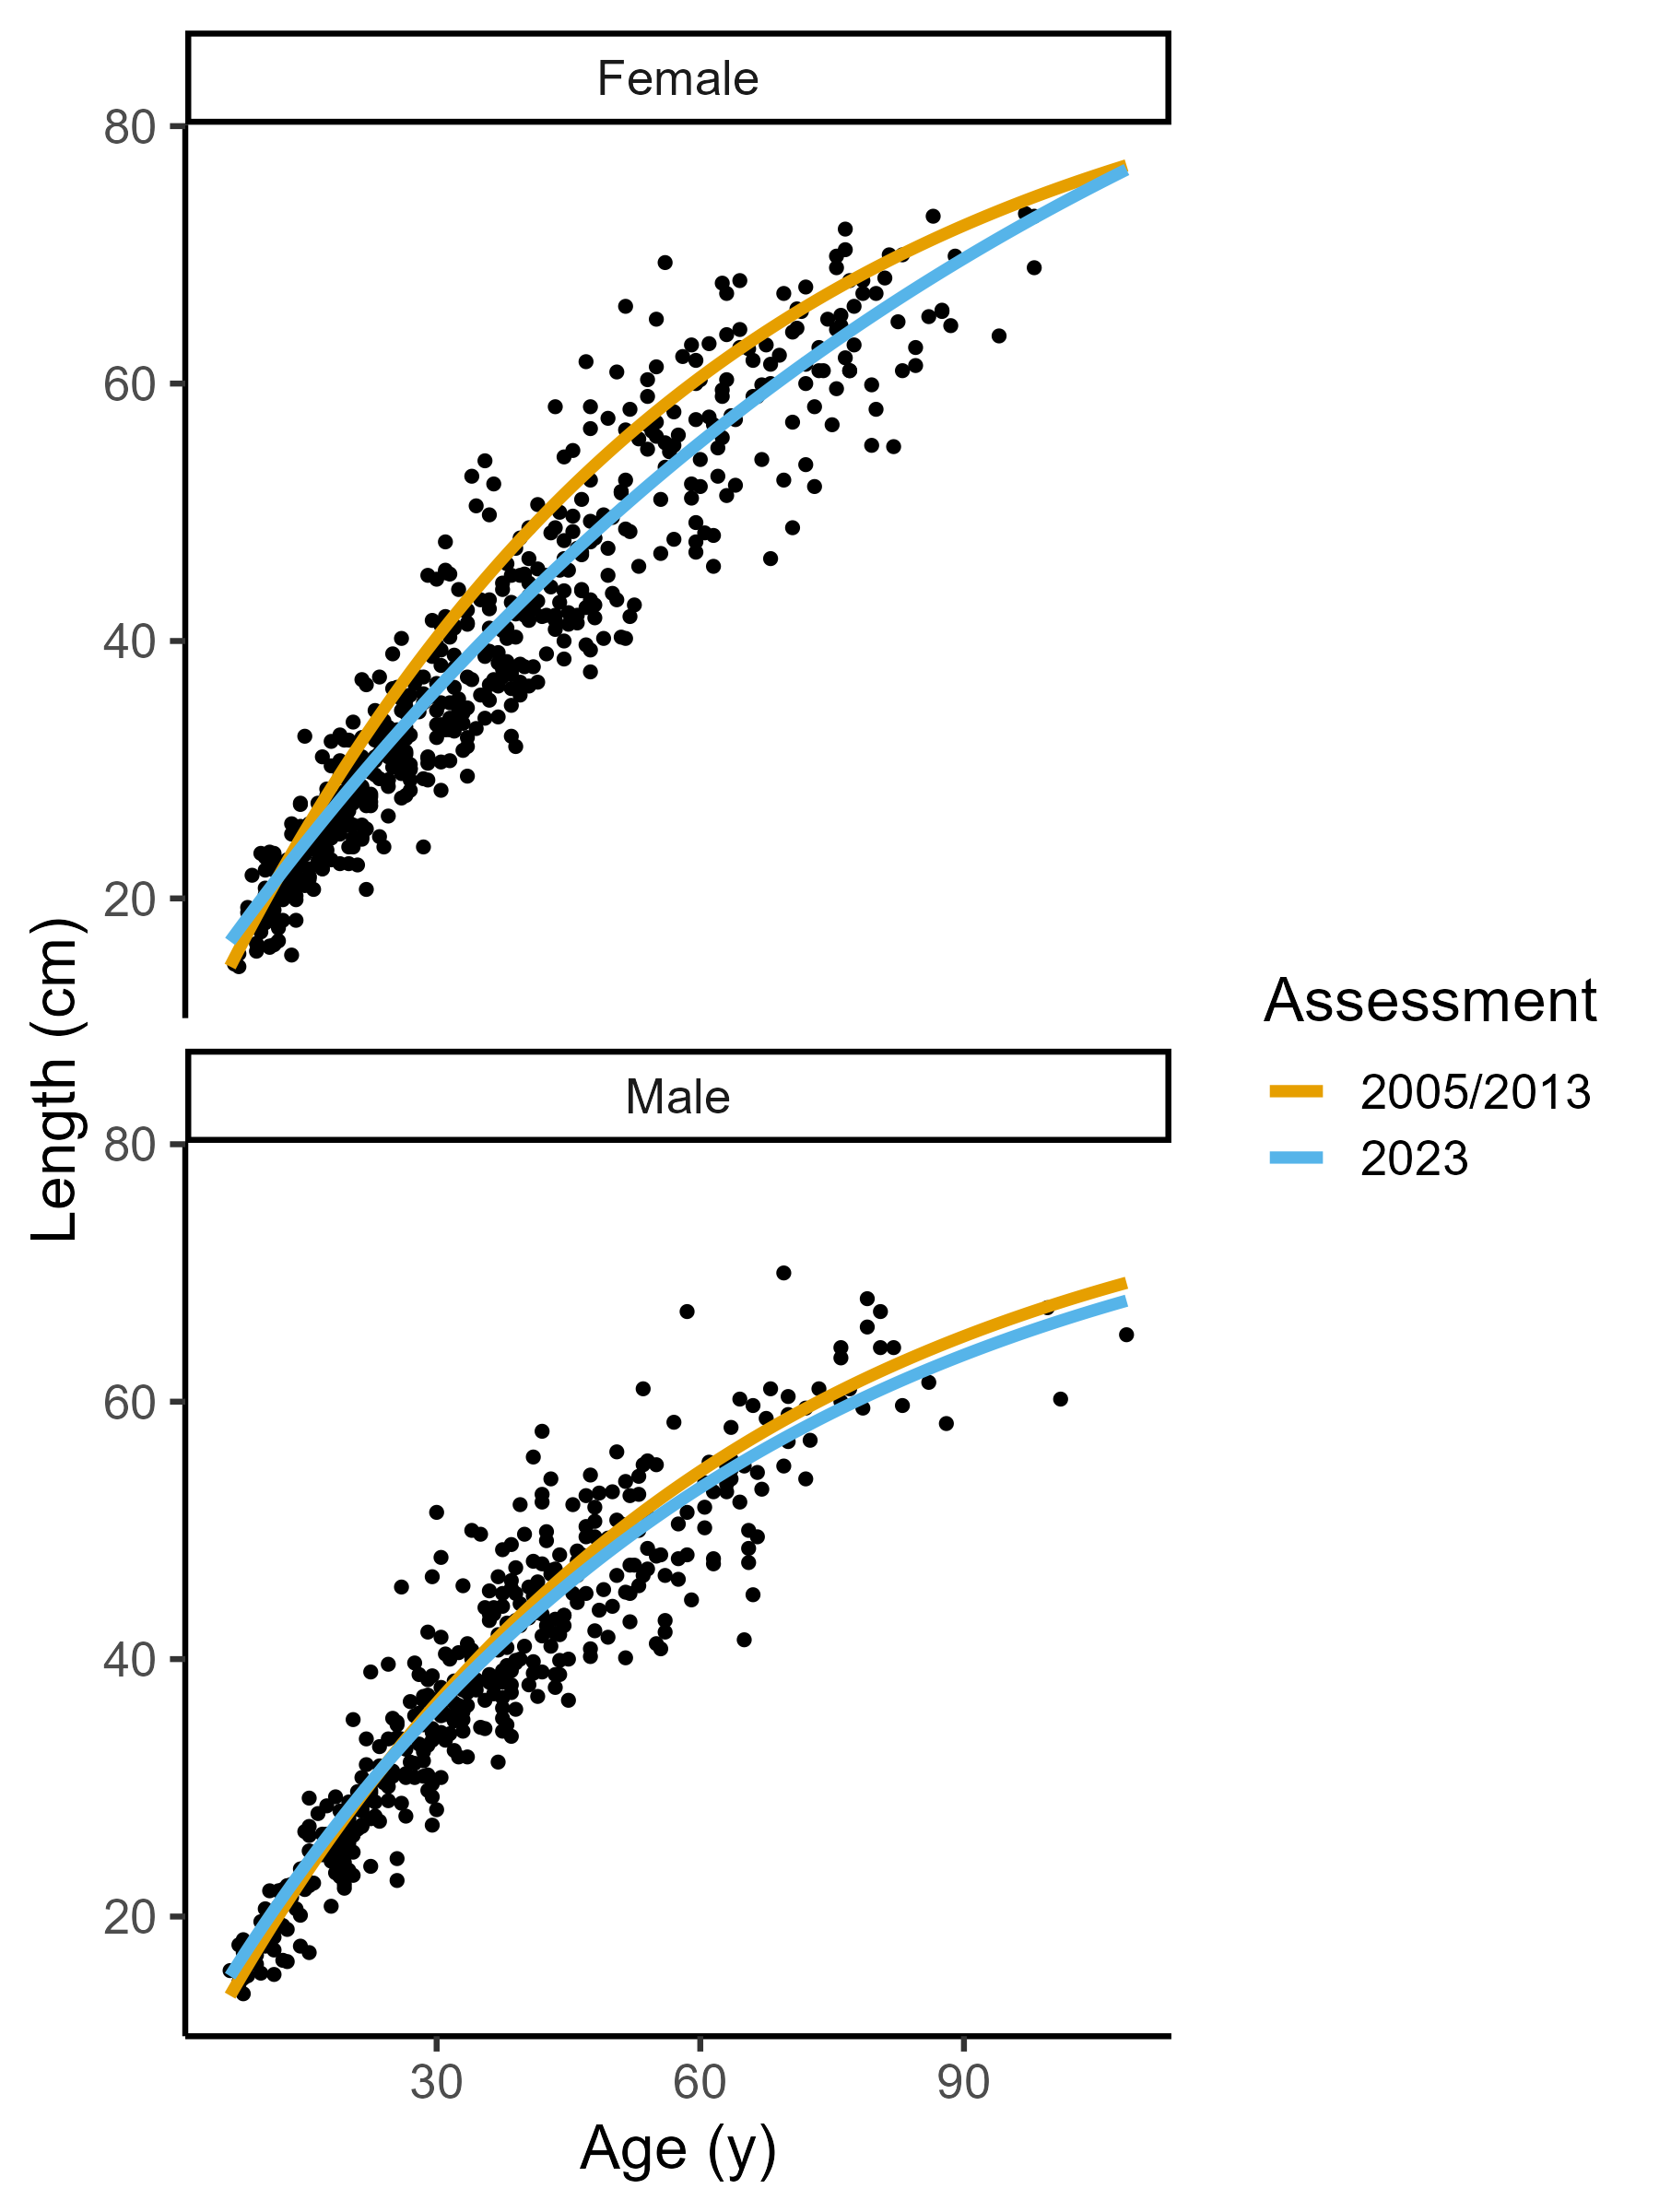
\includegraphics[width=1\textwidth,height=1\textheight]{C:/GitHub/Official_shortspine_thornyhead_2023/doc/FinalFigs/Data/growth_curve_comparison_LAA1.png}
\caption{Growth curve comparison. .\label{fig:growth_LAA1}}
\end{figure}

\begin{figure}
\centering
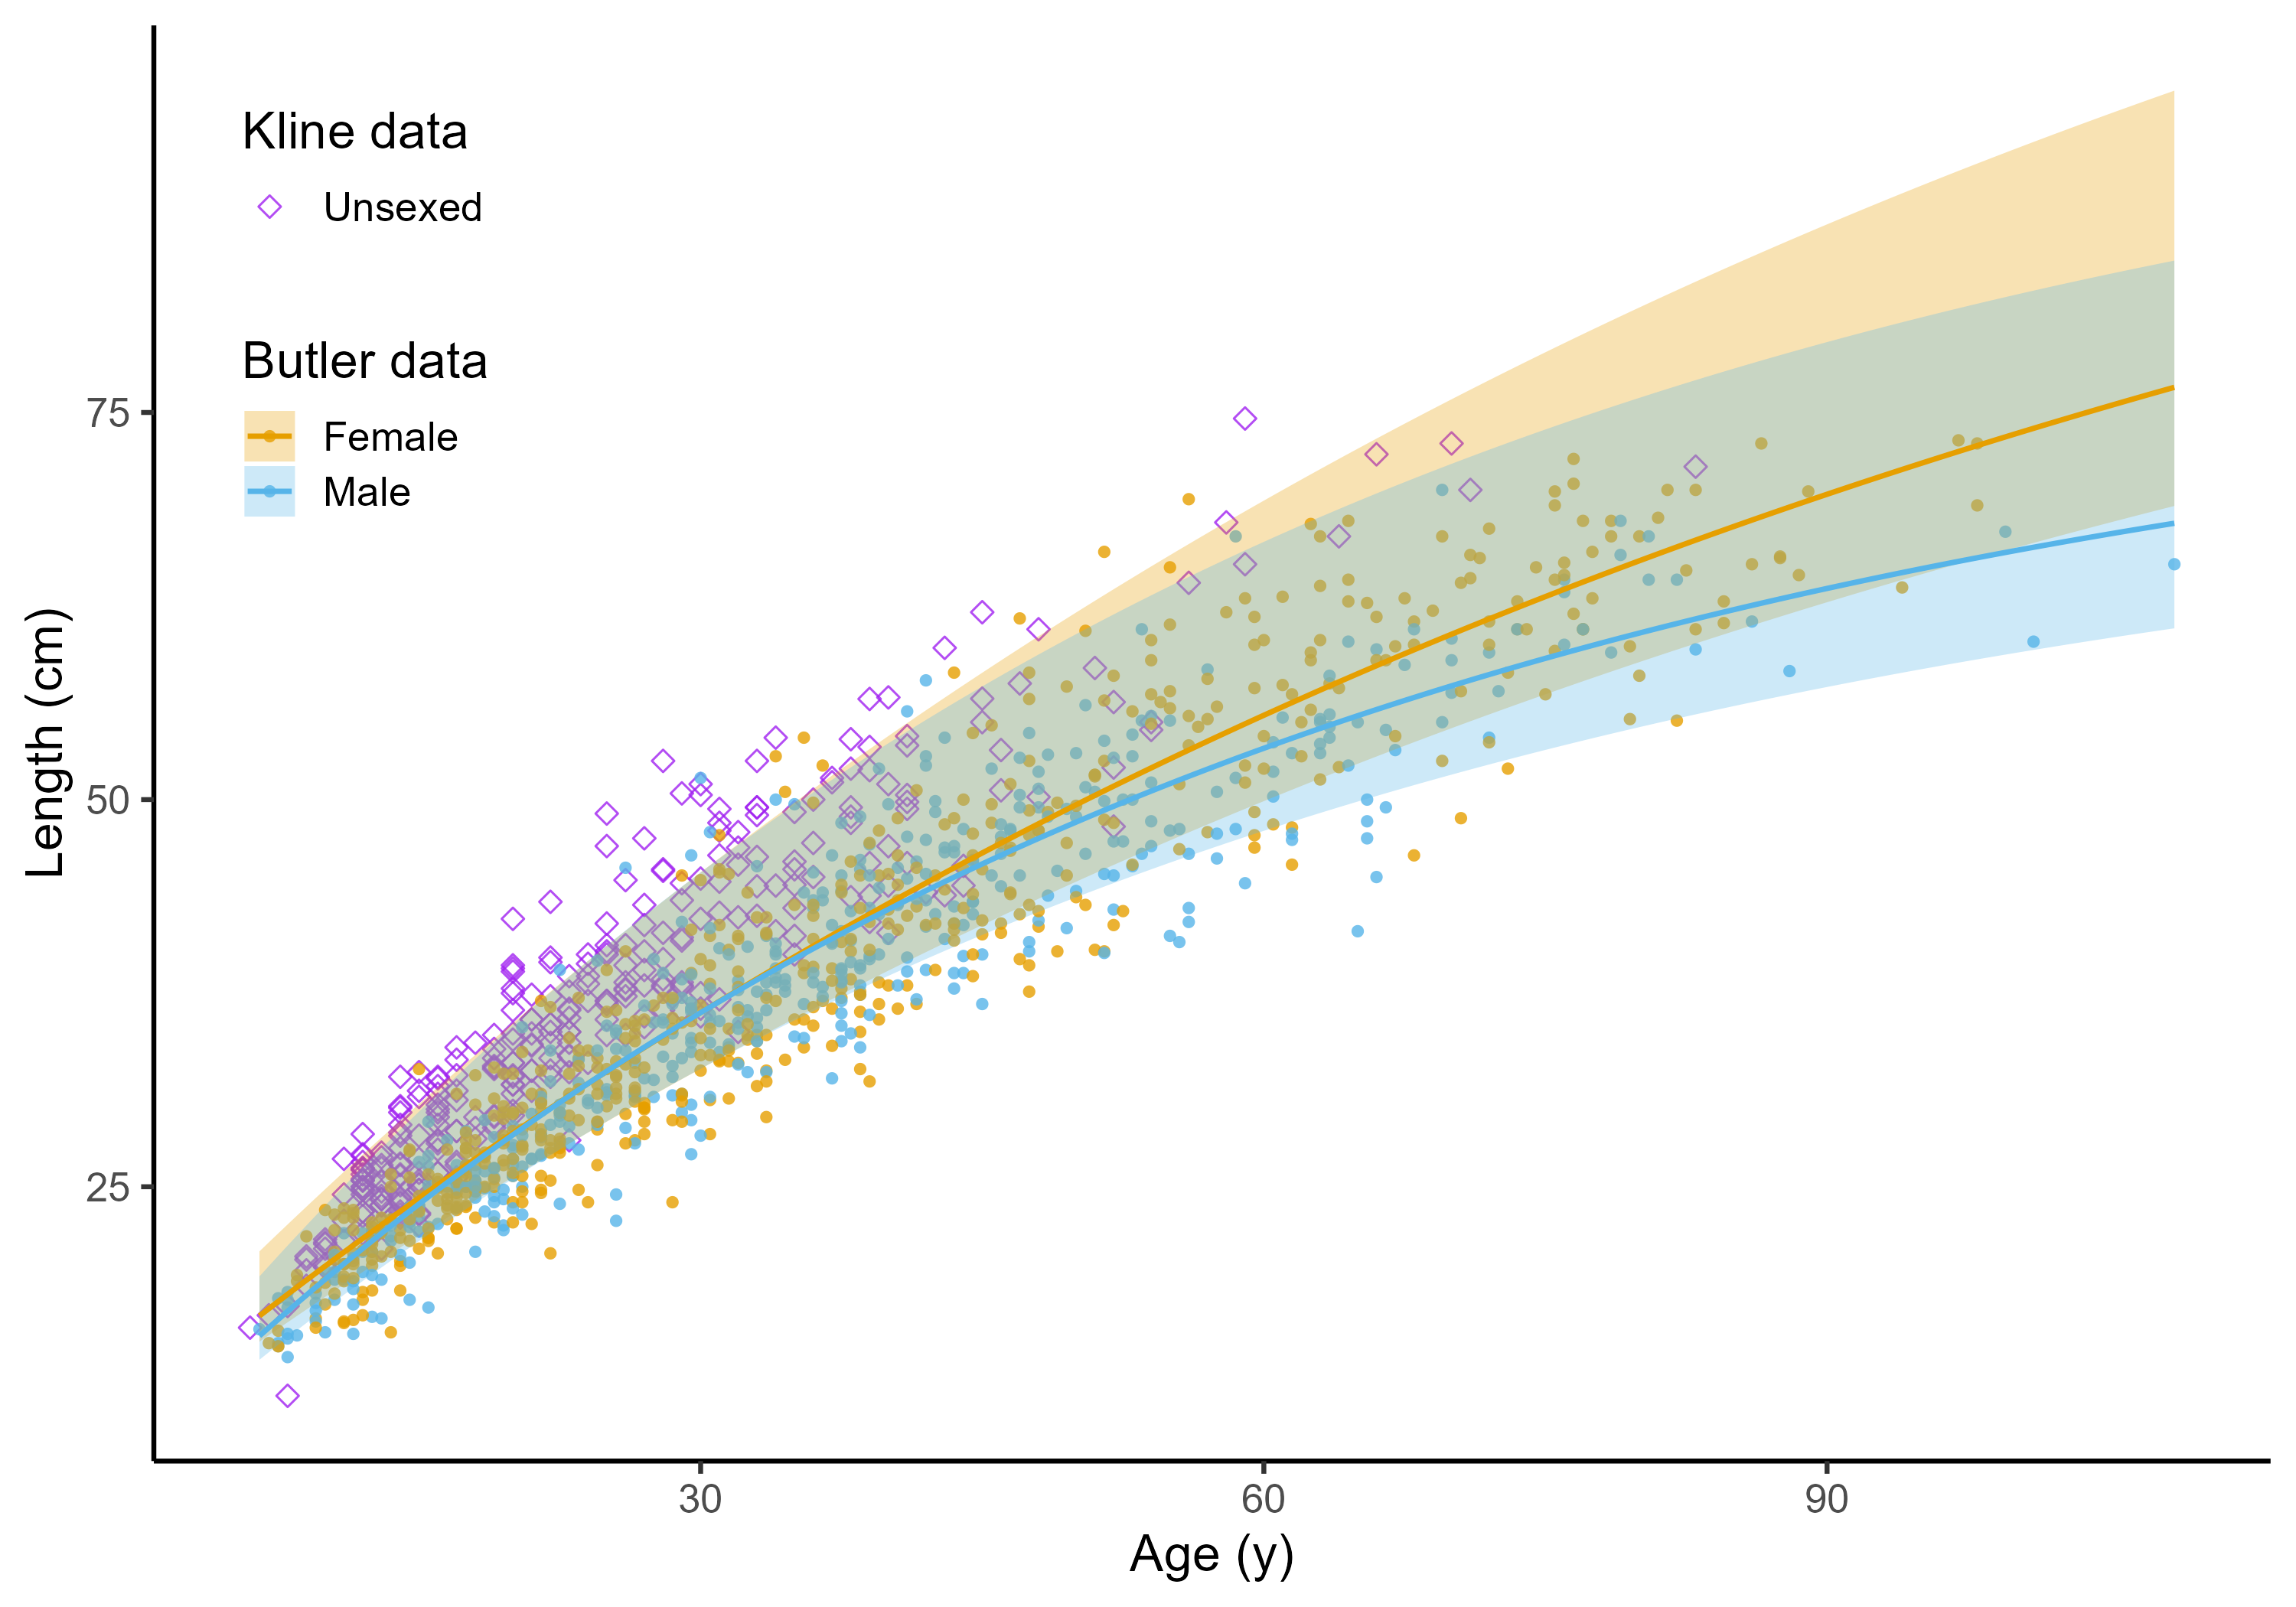
\includegraphics[width=1\textwidth,height=1\textheight]{C:/GitHub/Official_shortspine_thornyhead_2023/doc/FinalFigs/Data/growth_curve_sensitivities_LAA2.png}
\caption{Growth curve sensitivities.\label{fig:growth_LAA2}}
\end{figure}
\end{document}
